%%%%%%%%%%%%  Generated using docx2latex.com  %%%%%%%%%%%%%%

%%%%%%%%%%%%  v2.0.0-beta  %%%%%%%%%%%%%%

\documentclass[12pt]{report}
\usepackage{amsmath}
\usepackage{latexsym}
\usepackage{amsfonts}
\usepackage[normalem]{ulem}
\usepackage{soul}
\usepackage{array}
\usepackage{amssymb}
\usepackage{extarrows}
\usepackage{graphicx}
\usepackage[backend=biber,
style=numeric,
sorting=none,
isbn=false,
doi=false,
url=false,
]{biblatex}\addbibresource{bibliography.bib}

\usepackage{subfig}
\usepackage{wrapfig}
\usepackage{wasysym}
\usepackage{enumitem}
\usepackage{adjustbox}
\usepackage{ragged2e}
\usepackage[svgnames,table]{xcolor}
\usepackage{tikz}
\usepackage{longtable}
\usepackage{changepage}
\usepackage{setspace}
\usepackage{hhline}
\usepackage{multicol}
\usepackage{tabto}
\usepackage{float}
\usepackage{multirow}
\usepackage{makecell}
\usepackage{fancyhdr}
\usepackage[toc,page]{appendix}
\usepackage[hidelinks]{hyperref}
\usetikzlibrary{shapes.symbols,shapes.geometric,shadows,arrows.meta}
\tikzset{>={Latex[width=1.5mm,length=2mm]}}
\usepackage{flowchart}\usepackage[paperheight=11.0in,paperwidth=8.5in,left=1.38in,right=0.79in,top=1.18in,bottom=0.79in,headheight=1in]{geometry}
\usepackage[utf8]{inputenc}
\usepackage[T1]{fontenc}
\TabPositions{0.49in,0.98in,1.47in,1.96in,2.45in,2.94in,3.43in,3.92in,4.41in,4.9in,5.39in,5.88in,}

\urlstyle{same}


 %%%%%%%%%%%%  Set Depths for Sections  %%%%%%%%%%%%%%

% 1) Section
% 1.1) SubSection
% 1.1.1) SubSubSection
% 1.1.1.1) Paragraph
% 1.1.1.1.1) Subparagraph


\setcounter{tocdepth}{5}
\setcounter{secnumdepth}{5}


 %%%%%%%%%%%%  Set Depths for Nested Lists created by \begin{enumerate}  %%%%%%%%%%%%%%


\setlistdepth{9}
\renewlist{enumerate}{enumerate}{9}
		\setlist[enumerate,1]{label=\arabic*)}
		\setlist[enumerate,2]{label=\alph*)}
		\setlist[enumerate,3]{label=(\roman*)}
		\setlist[enumerate,4]{label=(\arabic*)}
		\setlist[enumerate,5]{label=(\Alph*)}
		\setlist[enumerate,6]{label=(\Roman*)}
		\setlist[enumerate,7]{label=\arabic*}
		\setlist[enumerate,8]{label=\alph*}
		\setlist[enumerate,9]{label=\roman*}

\renewlist{itemize}{itemize}{9}
		\setlist[itemize]{label=$\cdot$}
		\setlist[itemize,1]{label=\textbullet}
		\setlist[itemize,2]{label=$\circ$}
		\setlist[itemize,3]{label=$\ast$}
		\setlist[itemize,4]{label=$\dagger$}
		\setlist[itemize,5]{label=$\triangleright$}
		\setlist[itemize,6]{label=$\bigstar$}
		\setlist[itemize,7]{label=$\blacklozenge$}
		\setlist[itemize,8]{label=$\prime$}



 %%%%%%%%%%%%  Header here  %%%%%%%%%%%%%%


\pagestyle{fancy}
\fancyhf{}
\chead{ 

%%%%%%%%%%%%%%%%%%%% Figure/Image No: 1 starts here %%%%%%%%%%%%%%%%%%%%

\begin{figure}[H]
\advance\leftskip -0.55in		\includegraphics[width=0.47in,height=0.64in]{./../customXml/item1.xml}
\end{figure}


%%%%%%%%%%%%%%%%%%%% Figure/Image No: 1 Ends here %%%%%%%%%%%%%%%%%%%%

ChatBot Life\par 
 \begin{tikzpicture}

\draw (0.0in,0.0in) -- (6.12in,-0.0in); 
}
\cfoot{ 
\end{tikzpicture}

\vspace{\baselineskip}
}
\renewcommand{\headrulewidth}{0pt}
\setlength{\topsep}{0pt}\setlength{\parskip}{9.96pt}
\setlength{\parindent}{0pt}

 %%%%%%%%%%%%  This sets linespacing (verticle gap between Lines) Default=1 %%%%%%%%%%%%%%


\renewcommand{\arraystretch}{1.3}


%%%%%%%%%%%%%%%%%%%% Document code starts here %%%%%%%%%%%%%%%%%%%%



\begin{document}


%%%%%%%%%%%%%%%%%%%% Figure/Image No: 2 starts here %%%%%%%%%%%%%%%%%%%%

\begin{figure}[H]
	\begin{Center}
		
\includegraphics[width=1.09in,height=1.46in]{./media/image1.png}
	\end{Center}
\end{figure}


%%%%%%%%%%%%%%%%%%%% Figure/Image No: 2 Ends here %%%%%%%%%%%%%%%%%%%%

\setlength{\parskip}{0.0pt}
\par


\vspace{\baselineskip}
\begin{Center}
{\fontsize{18pt}{21.6pt}\selectfont \textbf{UNIVERSIDAD PRIVADA DE TACNA}\par}
\end{Center}\par


\vspace{\baselineskip}
\begin{Center}
{\fontsize{16pt}{19.2pt}\selectfont \textbf{FACULTAD DE INGENIERIA}\par}
\end{Center}\par

\begin{Center}
{\fontsize{16pt}{19.2pt}\selectfont \textbf{Escuela Profesional de Ingeniería de Sistemas}\par}
\end{Center}\par


\vspace{\baselineskip}

\vspace{\baselineskip}
\begin{Center}
{\fontsize{18pt}{21.6pt}\selectfont \textbf{CHATBOT FAING}\par}
\end{Center}\par


\vspace{\baselineskip}
\begin{Center}
{\fontsize{16pt}{19.2pt}\selectfont Curso: Inteligencia de Negocios\par}
\end{Center}\par


\vspace{\baselineskip}

\vspace{\baselineskip}
\begin{Center}
{\fontsize{16pt}{19.2pt}\selectfont Docente: Ing. Patrick Cuadros Quiroga\par}
\end{Center}\par


\vspace{\baselineskip}
{\fontsize{16pt}{19.2pt}\selectfont Integrantes:\par}\par


\vspace{\baselineskip}
{\fontsize{16pt}{19.2pt}\selectfont \textbf{Núñez Mamani, Samuel Ray\tab \tab \tab \tab (2016054462)}\par}\par

{\fontsize{16pt}{19.2pt}\selectfont \textbf{Reinoso Aranda,Andre Sebastián\tab \tab (2016055275)}\par}\par

{\fontsize{16pt}{19.2pt}\selectfont \textbf{De La Barra Vasquez, Andres Eduardo\tab (2016055087)}\par}\par

\begin{adjustwidth}{0.49in}{0.0in}
{\fontsize{16pt}{19.2pt}\selectfont \textbf{Damian Mamani, David Reynaldo\tab \tab (2016055194)}\par}\par

\end{adjustwidth}


\vspace{\baselineskip}

\vspace{\baselineskip}

\vspace{\baselineskip}

\vspace{\baselineskip}

\vspace{\baselineskip}

\vspace{\baselineskip}
\begin{Center}
{\fontsize{16pt}{19.2pt}\selectfont \textbf{Tacna – Perú}\par}
\end{Center}\par

\begin{Center}
{\fontsize{16pt}{19.2pt}\selectfont \textbf{2018}\par}
\end{Center}\par


\vspace{\baselineskip}
\setlength{\parskip}{9.96pt}


 %%%%%%%%%%%%  Starting New Page here %%%%%%%%%%%%%%

\newpage

\vspace{\baselineskip}\setlength{\parskip}{0.0pt}
\begin{Center}
\textbf{INDICE GENERAL}
\end{Center}\par


\vspace{\baselineskip}


 %%%%%%%%%%%%  This Produces Table Of Contents %%%%%%%%%%%%%%

\tableofcontents
\addcontentsline{toc}{chapter}{Contents}

\vspace{\baselineskip}\setlength{\parskip}{9.96pt}


 %%%%%%%%%%%%  Starting New Page here %%%%%%%%%%%%%%

\newpage

\vspace{\baselineskip}\section*{CHATBOT LIFE}
\addcontentsline{toc}{section}{CHATBOT LIFE}
\setlength{\parskip}{0.0pt}
\begin{enumerate}
	\item \textbf{EMPRESA}
\end{enumerate}\par

\begin{enumerate}
	\item \textbf{Nombre:}\par

{\fontsize{10pt}{12.0pt}\selectfont BeProgrammer\par}\par


\vspace{\baselineskip}
	\item \textbf{Rubro:}\par

{\fontsize{10pt}{12.0pt}\selectfont Empresa dedicada a la creación de software de aplicación totalmente con menores costos a los que están presentes en el mercado.\par}\par


\vspace{\baselineskip}

\end{enumerate}
	\item \textbf{LINEA DE INVESTIGACION:}\par



%%%%%%%%%%%%%%%%%%%% Figure/Image No: 3 starts here %%%%%%%%%%%%%%%%%%%%

\begin{figure}[H]
\advance\leftskip -0.07in		
\includegraphics[width=2.73in,height=2.21in]{./media/image2.jpeg}
\end{figure}


%%%%%%%%%%%%%%%%%%%% Figure/Image No: 3 Ends here %%%%%%%%%%%%%%%%%%%%



 %%%%%%%%%%%%  Starting New Page here %%%%%%%%%%%%%%

\newpage

\vspace{\baselineskip}\setlength{\parskip}{0.0pt}
\begin{enumerate}
	\item \textbf{DESARROLLO DE LA SOLUCION:}\par


\end{enumerate}\subsection*{7.1\hspace*{10pt}Factibilidad del proyecto:}
\addcontentsline{toc}{subsection}{7.1\hspace*{10pt}Factibilidad del proyecto:}
\begin{itemize}
	\item {\fontsize{10pt}{12.0pt}\selectfont Técnica\par}\par

{\fontsize{10pt}{12.0pt}\selectfont El desarrollo del software está siendo efectuado por personas que han investigado todo lo posible a cerca del tema. Buscando satisfacer la necesidad de solucionar la problemática presente, en este caso a dificultad de los alumnos de poder tener un acceso rápido y eficaz a lo que concierne a tu entorno estudiantil ya sea los eventos o hasta simples números de teléfono.\par}\par


\vspace{\baselineskip}
	\item {\fontsize{10pt}{12.0pt}\selectfont Económica\par}\par

{\fontsize{10pt}{12.0pt}\selectfont En el caso de querer implementar un Chatbot en la plataforma de Microsoft Azure, se tiene un costo por mensajes enviados y recibidos, Las dos tarifas básicas son: Standart y Free, En el caso del plan de tarifa Free nos da la opción de poder ejecutar 10000 mensajes a comparación del servicio estándar.\par}\par



%%%%%%%%%%%%%%%%%%%% Figure/Image No: 4 starts here %%%%%%%%%%%%%%%%%%%%

\begin{figure}[H]
	\begin{Center}
		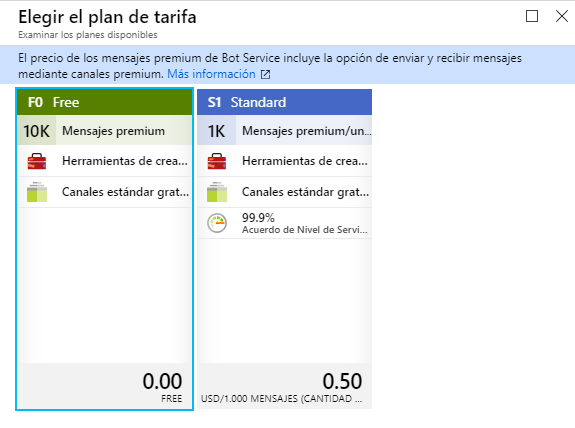
\includegraphics[width=5.23in,height=3.9in]{./media/image3.png}
	\end{Center}
\end{figure}


%%%%%%%%%%%%%%%%%%%% Figure/Image No: 4 Ends here %%%%%%%%%%%%%%%%%%%%

\par

	\item {\fontsize{10pt}{12.0pt}\selectfont Operativa\par}
\end{itemize}\par

{\fontsize{10pt}{12.0pt}\selectfont El uso del chatbot propuesto depende de la insentivacion del mismo, propaganda o anuncio de la misma, para poder llegar a todo el público objetivo, en este caso los alumnos que están estudiando en la facultad.\par}\par

{\fontsize{10pt}{12.0pt}\selectfont El uso de tecnología nuevas para una empresa u organización puede ser difícil si no se trata con la debida responsabilidad.\par}\par

\subsection*{7.2\hspace*{10pt}Alcance y Limites:}
\addcontentsline{toc}{subsection}{7.2\hspace*{10pt}Alcance y Limites:}
\begin{itemize}
	\item {\fontsize{10pt}{12.0pt}\selectfont Alcance\par}\par

{\fontsize{10pt}{12.0pt}\selectfont Se espera que el sistema pueda ser operado por todos los estudiantes, y consultado desde su Smartphone.\par}\par


\vspace{\baselineskip}
	\item {\fontsize{10pt}{12.0pt}\selectfont Limites\par}
\end{itemize}\par

\begin{adjustwidth}{1.0in}{0.0in}
{\fontsize{10pt}{12.0pt}\selectfont La\ frontera del sistema está delimitada por la conexión a internet, pues la información del ChatBot se provee desde la base de datos, la que está alojada en la  nube de Azure.\par}\par

\end{adjustwidth}


\vspace{\baselineskip}
\subsection*{7.3\hspace*{10pt}Requerimientos Funcionales y No funcionales:}
\addcontentsline{toc}{subsection}{7.3\hspace*{10pt}Requerimientos Funcionales y No funcionales:}
\begin{itemize}
	\item {\fontsize{10pt}{12.0pt}\selectfont Requerimientos Funcionales\par}\par



%%%%%%%%%%%%%%%%%%%% Table No: 1 starts here %%%%%%%%%%%%%%%%%%%%


\begin{table}[H]
 			\centering
\begin{tabular}{p{0.26in}p{3.33in}p{1.8in}}
\hline
%row no:1
\multicolumn{1}{|p{0.26in}}{{\fontsize{10pt}{12.0pt}\selectfont ID}} & 
\multicolumn{1}{|p{3.33in}}{{\fontsize{10pt}{12.0pt}\selectfont Descripción}} & 
\multicolumn{1}{|p{1.8in}|}{{\fontsize{10pt}{12.0pt}\selectfont Caso de Uso}} \\
\hhline{---}
%row no:2
\multicolumn{1}{|p{0.26in}}{{\fontsize{10pt}{12.0pt}\selectfont 1}} & 
\multicolumn{1}{|p{3.33in}}{{\fontsize{10pt}{12.0pt}\selectfont CRUD persona se crea para poder a los docentes y delegados}} & 
\multicolumn{1}{|p{1.8in}|}{{\fontsize{10pt}{12.0pt}\selectfont CRUD persona}} \\
\hhline{---}
%row no:3
\multicolumn{1}{|p{0.26in}}{{\fontsize{10pt}{12.0pt}\selectfont 2}} & 
\multicolumn{1}{|p{3.33in}}{{\fontsize{10pt}{12.0pt}\selectfont CRUD docente que podrá introducir temas a los cursos}} & 
\multicolumn{1}{|p{1.8in}|}{{\fontsize{10pt}{12.0pt}\selectfont CRUD docente}} \\
\hhline{---}
%row no:4
\multicolumn{1}{|p{0.26in}}{{\fontsize{10pt}{12.0pt}\selectfont 3}} & 
\multicolumn{1}{|p{3.33in}}{{\fontsize{10pt}{12.0pt}\selectfont CRUD delegado que podrá introducir temas a los cursos}} & 
\multicolumn{1}{|p{1.8in}|}{{\fontsize{10pt}{12.0pt}\selectfont CRUD delegado}} \\
\hhline{---}
%row no:5
\multicolumn{1}{|p{0.26in}}{{\fontsize{10pt}{12.0pt}\selectfont 4}} & 
\multicolumn{1}{|p{3.33in}}{{\fontsize{10pt}{12.0pt}\selectfont CRUD usuario que pueden ingresar al sistema que controla el flujo de datos}} & 
\multicolumn{1}{|p{1.8in}|}{{\fontsize{10pt}{12.0pt}\selectfont CRUD usuario}} \\
\hhline{---}
%row no:6
\multicolumn{1}{|p{0.26in}}{{\fontsize{10pt}{12.0pt}\selectfont 5}} & 
\multicolumn{1}{|p{3.33in}}{{\fontsize{10pt}{12.0pt}\selectfont CRUD escuela creada por los usuarios administradores}} & 
\multicolumn{1}{|p{1.8in}|}{{\fontsize{10pt}{12.0pt}\selectfont CRUD escuela}} \\
\hhline{---}
%row no:7
\multicolumn{1}{|p{0.26in}}{{\fontsize{10pt}{12.0pt}\selectfont 6}} & 
\multicolumn{1}{|p{3.33in}}{{\fontsize{10pt}{12.0pt}\selectfont CRUD curso creado para las escuelas}} & 
\multicolumn{1}{|p{1.8in}|}{{\fontsize{10pt}{12.0pt}\selectfont CRUD curso}} \\
\hhline{---}
%row no:8
\multicolumn{1}{|p{0.26in}}{{\fontsize{10pt}{12.0pt}\selectfont 7}} & 
\multicolumn{1}{|p{3.33in}}{{\fontsize{10pt}{12.0pt}\selectfont CRUD evento creadas por los usuarios siendo mostradas por el chat cuando estén activos}} & 
\multicolumn{1}{|p{1.8in}|}{{\fontsize{10pt}{12.0pt}\selectfont CRUD evento}} \\
\hhline{---}
%row no:9
\multicolumn{1}{|p{0.26in}}{{\fontsize{10pt}{12.0pt}\selectfont 8}} & 
\multicolumn{1}{|p{3.33in}}{{\fontsize{10pt}{12.0pt}\selectfont CRUD teléfono de las escuelas}} & 
\multicolumn{1}{|p{1.8in}|}{{\fontsize{10pt}{12.0pt}\selectfont CRUD teléfono}} \\
\hhline{---}
%row no:10
\multicolumn{1}{|p{0.26in}}{{\fontsize{10pt}{12.0pt}\selectfont 9}} & 
\multicolumn{1}{|p{3.33in}}{{\fontsize{10pt}{12.0pt}\selectfont CRUD tema de estudio que pueden ser creadas por los delegados o por los docente}} & 
\multicolumn{1}{|p{1.8in}|}{{\fontsize{10pt}{12.0pt}\selectfont CRUD tema}} \\
\hhline{---}
%row no:11
\multicolumn{1}{|p{0.26in}}{{\fontsize{10pt}{12.0pt}\selectfont 10}} & 
\multicolumn{1}{|p{3.33in}}{{\fontsize{10pt}{12.0pt}\selectfont El usuario debe de ingresar un mensaje dependiendo del listado que se muestre en la pantalla. Una vez seguido los pasos el mensaje será interpretado por LUIS y esto producirá la respuesta según la consulta}} & 
\multicolumn{1}{|p{1.8in}|}{{\fontsize{10pt}{12.0pt}\selectfont Ejecutar consulta}} \\
\hhline{---}

\end{tabular}
 \end{table}


%%%%%%%%%%%%%%%%%%%% Table No: 1 ends here %%%%%%%%%%%%%%%%%%%%


\vspace{\baselineskip}

\vspace{\baselineskip}
	\item {\fontsize{10pt}{12.0pt}\selectfont Requerimientos No Funcionales\par}
\end{itemize}\par



%%%%%%%%%%%%%%%%%%%% Table No: 2 starts here %%%%%%%%%%%%%%%%%%%%


\begin{table}[H]
 			\centering
\begin{tabular}{p{1.96in}p{1.96in}p{1.96in}}
\hline
%row no:1
\multicolumn{1}{|p{1.96in}}{\Centering {\fontsize{10pt}{12.0pt}\selectfont ID}} & 
\multicolumn{1}{|p{1.96in}}{\Centering {\fontsize{10pt}{12.0pt}\selectfont Requerimiento No funcional}} & 
\multicolumn{1}{|p{1.96in}|}{\Centering {\fontsize{10pt}{12.0pt}\selectfont Descripción}} \\
\hhline{---}
%row no:2
\multicolumn{1}{|p{1.96in}}{\Centering {\fontsize{10pt}{12.0pt}\selectfont 1}} & 
\multicolumn{1}{|p{1.96in}}{\Centering {\fontsize{10pt}{12.0pt}\selectfont Usabilidad}} & 
\multicolumn{1}{|p{1.96in}|}{\Centering {\fontsize{10pt}{12.0pt}\selectfont Formularios intuitivos }} \\
\hhline{---}
%row no:3
\multicolumn{1}{|p{1.96in}}{\Centering {\fontsize{10pt}{12.0pt}\selectfont 2}} & 
\multicolumn{1}{|p{1.96in}}{\Centering {\fontsize{10pt}{12.0pt}\selectfont Disponibilidad}} & 
\multicolumn{1}{|p{1.96in}|}{\Centering {\fontsize{10pt}{12.0pt}\selectfont La Base de datos está disponible las 24/7}} \\
\hhline{---}
%row no:4
\multicolumn{1}{|p{1.96in}}{\Centering {\fontsize{10pt}{12.0pt}\selectfont 3}} & 
\multicolumn{1}{|p{1.96in}}{\Centering {\fontsize{10pt}{12.0pt}\selectfont Disponibilidad}} & 
\multicolumn{1}{|p{1.96in}|}{\Centering {\fontsize{10pt}{12.0pt}\selectfont El sistema está disponible 24/7}} \\
\hhline{---}
%row no:5
\multicolumn{1}{|p{1.96in}}{\Centering {\fontsize{10pt}{12.0pt}\selectfont 4}} & 
\multicolumn{1}{|p{1.96in}}{\Centering {\fontsize{10pt}{12.0pt}\selectfont Rendimiento}} & 
\multicolumn{1}{|p{1.96in}|}{\Centering El sistema funciona con gran cantidad de información en sus procesos} \\
\hhline{---}
%row no:6
\multicolumn{1}{|p{1.96in}}{\Centering {\fontsize{10pt}{12.0pt}\selectfont 5}} & 
\multicolumn{1}{|p{1.96in}}{\Centering {\fontsize{10pt}{12.0pt}\selectfont Desempeño}} & 
\multicolumn{1}{|p{1.96in}|}{\Centering {\fontsize{10pt}{12.0pt}\selectfont Pensado en Pc de bajo rendimiento}} \\
\hhline{---}
%row no:7
\multicolumn{1}{|p{1.96in}}{\Centering {\fontsize{10pt}{12.0pt}\selectfont 6}} & 
\multicolumn{1}{|p{1.96in}}{\Centering {\fontsize{10pt}{12.0pt}\selectfont Desempeño}} & 
\multicolumn{1}{|p{1.96in}|}{\Centering El sistema no presentara problemas en su ejecución} \\
\hhline{---}
%row no:8
\multicolumn{1}{|p{1.96in}}{\Centering {\fontsize{10pt}{12.0pt}\selectfont 7}} & 
\multicolumn{1}{|p{1.96in}}{\Centering {\fontsize{10pt}{12.0pt}\selectfont Desempeño}} & 
\multicolumn{1}{|p{1.96in}|}{\Centering La base de datos debe maneja de responderá a las exigencia del sistema} \\
\hhline{---}
%row no:9
\multicolumn{1}{|p{1.96in}}{\Centering {\fontsize{10pt}{12.0pt}\selectfont 8}} & 
\multicolumn{1}{|p{1.96in}}{\Centering {\fontsize{10pt}{12.0pt}\selectfont Seguridad}} & 
\multicolumn{1}{|p{1.96in}|}{\Centering {\fontsize{10pt}{12.0pt}\selectfont Login para ingresar al sistema}} \\
\hhline{---}
%row no:10
\multicolumn{1}{|p{1.96in}}{\Centering {\fontsize{10pt}{12.0pt}\selectfont 9}} & 
\multicolumn{1}{|p{1.96in}}{\Centering {\fontsize{10pt}{12.0pt}\selectfont Disponibilidad}} & 
\multicolumn{1}{|p{1.96in}|}{\Centering {\fontsize{10pt}{12.0pt}\selectfont El ChatBot debe de estar disponible 24/7}} \\
\hhline{---}
%row no:11
\multicolumn{1}{|p{1.96in}}{\Centering {\fontsize{10pt}{12.0pt}\selectfont 10}} & 
\multicolumn{1}{|p{1.96in}}{\Centering {\fontsize{10pt}{12.0pt}\selectfont Desempeño}} & 
\multicolumn{1}{|p{1.96in}|}{\Centering {\fontsize{10pt}{12.0pt}\selectfont El bot responderá las necesidades de los usuarios correspondiente a sus dudas}} \\
\hhline{---}
%row no:12
\multicolumn{1}{|p{1.96in}}{\Centering {\fontsize{10pt}{12.0pt}\selectfont 11}} & 
\multicolumn{1}{|p{1.96in}}{\Centering {\fontsize{10pt}{12.0pt}\selectfont Plataforma}} & 
\multicolumn{1}{|p{1.96in}|}{\Centering El sistema está disponible en múltiples SO y al jdk 1.8} \\
\hhline{---}
%row no:13
\multicolumn{1}{|p{1.96in}}{\Centering {\fontsize{10pt}{12.0pt}\selectfont 12}} & 
\multicolumn{1}{|p{1.96in}}{\Centering {\fontsize{10pt}{12.0pt}\selectfont Plataforma}} & 
\multicolumn{1}{|p{1.96in}|}{\Centering {\fontsize{10pt}{12.0pt}\selectfont El bot se ejecuta en cualquier versión de Messenger}} \\
\hhline{---}

\end{tabular}
 \end{table}


%%%%%%%%%%%%%%%%%%%% Table No: 2 ends here %%%%%%%%%%%%%%%%%%%%


\vspace{\baselineskip}
\setlength{\parskip}{9.96pt}


 %%%%%%%%%%%%  Starting New Page here %%%%%%%%%%%%%%

\newpage

\vspace{\baselineskip}\subsection*{7.4\hspace*{10pt}Proceso:}
\addcontentsline{toc}{subsection}{7.4\hspace*{10pt}Proceso:}
\begin{itemize}
	\item {\fontsize{10pt}{12.0pt}\selectfont Diagrama de proceso propuesto\par}
\end{itemize}\par

\textbf{Login}\par



%%%%%%%%%%%%%%%%%%%% Figure/Image No: 5 starts here %%%%%%%%%%%%%%%%%%%%

\begin{figure}[H]
	\begin{Center}
		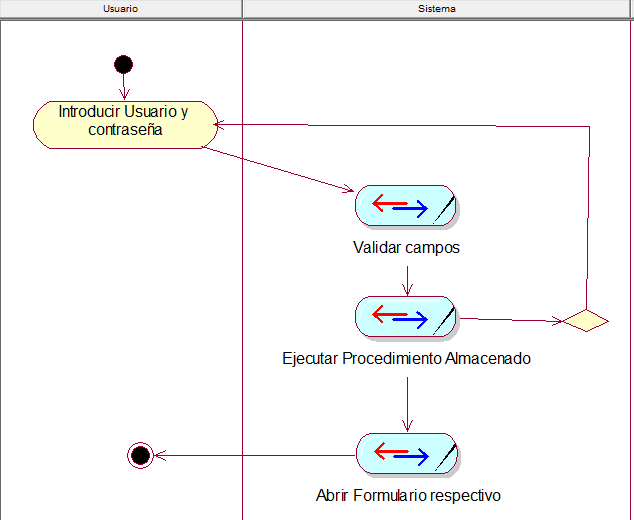
\includegraphics[width=5.08in,height=4.17in]{./media/image4.png}
	\end{Center}
\end{figure}


%%%%%%%%%%%%%%%%%%%% Figure/Image No: 5 Ends here %%%%%%%%%%%%%%%%%%%%

\par


\vspace{\baselineskip}

\vspace{\baselineskip}

\vspace{\baselineskip}


 %%%%%%%%%%%%  Starting New Page here %%%%%%%%%%%%%%

\newpage

\vspace{\baselineskip}\textbf{CRUD Diversos}\par



%%%%%%%%%%%%%%%%%%%% Figure/Image No: 6 starts here %%%%%%%%%%%%%%%%%%%%

\begin{figure}[H]
	\begin{Center}
		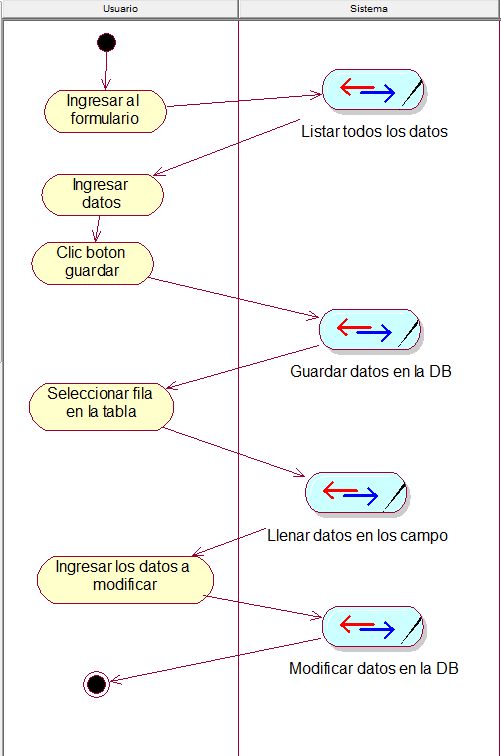
\includegraphics[width=4.62in,height=6.97in]{./media/image5.png}
	\end{Center}
\end{figure}


%%%%%%%%%%%%%%%%%%%% Figure/Image No: 6 Ends here %%%%%%%%%%%%%%%%%%%%

\par



 %%%%%%%%%%%%  Starting New Page here %%%%%%%%%%%%%%

\newpage

\vspace{\baselineskip}\textbf{ChatBot}\par



%%%%%%%%%%%%%%%%%%%% Figure/Image No: 7 starts here %%%%%%%%%%%%%%%%%%%%

\begin{figure}[H]
	\begin{Center}
		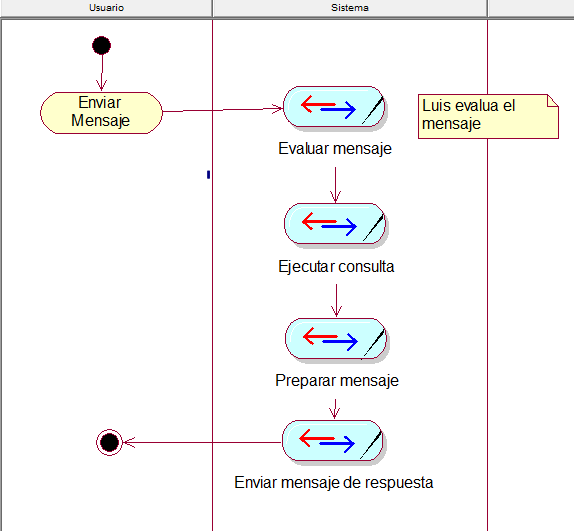
\includegraphics[width=4.84in,height=4.48in]{./media/image6.png}
	\end{Center}
\end{figure}


%%%%%%%%%%%%%%%%%%%% Figure/Image No: 7 Ends here %%%%%%%%%%%%%%%%%%%%

\par

\subsection*{7.5\hspace*{10pt}Especificación de casos de uso:}
\addcontentsline{toc}{subsection}{7.5\hspace*{10pt}Especificación de casos de uso:}
\begin{itemize}
	\item {\fontsize{10pt}{12.0pt}\selectfont Diagrama de casos de uso\par}\par



%%%%%%%%%%%%%%%%%%%% Figure/Image No: 8 starts here %%%%%%%%%%%%%%%%%%%%

\begin{figure}[H]
	\begin{Center}
		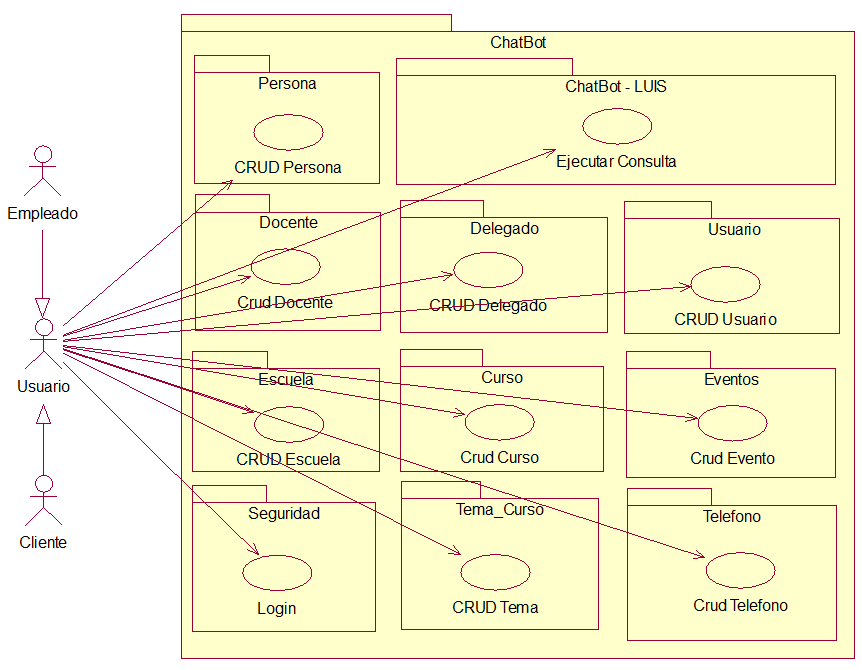
\includegraphics[width=4.23in,height=3.29in]{./media/image7.png}
	\end{Center}
\end{figure}


%%%%%%%%%%%%%%%%%%%% Figure/Image No: 8 Ends here %%%%%%%%%%%%%%%%%%%%

\par

	\item {\fontsize{10pt}{12.0pt}\selectfont Descripción de casos de uso\par}
\end{itemize}\par



%%%%%%%%%%%%%%%%%%%% Table No: 3 starts here %%%%%%%%%%%%%%%%%%%%


\begin{table}[H]
 			\centering
\begin{tabular}{p{1.15in}p{4.44in}}
\hline
%row no:1
\multicolumn{1}{|p{1.15in}}{{\fontsize{10pt}{12.0pt}\selectfont Caso de uso}} & 
\multicolumn{1}{|p{4.44in}|}{{\fontsize{10pt}{12.0pt}\selectfont Descripción}} \\
\hhline{--}
%row no:2
\multicolumn{1}{|p{1.15in}}{{\fontsize{10pt}{12.0pt}\selectfont CRUD Persona}} & 
\multicolumn{1}{|p{4.44in}|}{{\fontsize{10pt}{12.0pt}\selectfont Se guarda y se listan los datos ingresados para crear una persona}} \\
\hhline{--}
%row no:3
\multicolumn{1}{|p{1.15in}}{{\fontsize{10pt}{12.0pt}\selectfont CRUD Docente}} & 
\multicolumn{1}{|p{4.44in}|}{{\fontsize{10pt}{12.0pt}\selectfont Se debe de seleccionar una persona para poder crear un docente}} \\
\hhline{--}
%row no:4
\multicolumn{1}{|p{1.15in}}{{\fontsize{10pt}{12.0pt}\selectfont CRUD Delegado}} & 
\multicolumn{1}{|p{4.44in}|}{{\fontsize{10pt}{12.0pt}\selectfont Se debe de seleccionar una persona para poder crear un delegado}} \\
\hhline{--}
%row no:5
\multicolumn{1}{|p{1.15in}}{{\fontsize{10pt}{12.0pt}\selectfont CRUD Usuario}} & 
\multicolumn{1}{|p{4.44in}|}{{\fontsize{10pt}{12.0pt}\selectfont Se debe de seleccionar una persona para poder crear un usuario}} \\
\hhline{--}
%row no:6
\multicolumn{1}{|p{1.15in}}{{\fontsize{10pt}{12.0pt}\selectfont CRUD Escuela}} & 
\multicolumn{1}{|p{4.44in}|}{{\fontsize{10pt}{12.0pt}\selectfont Se guarda y se listan los datos ingresados para crear una escuela}} \\
\hhline{--}
%row no:7
\multicolumn{1}{|p{1.15in}}{{\fontsize{10pt}{12.0pt}\selectfont CRUD Curso}} & 
\multicolumn{1}{|p{4.44in}|}{{\fontsize{10pt}{12.0pt}\selectfont Se tiene que asignar un curso según la escuela}} \\
\hhline{--}
%row no:8
\multicolumn{1}{|p{1.15in}}{{\fontsize{10pt}{12.0pt}\selectfont CRUD Evento}} & 
\multicolumn{1}{|p{4.44in}|}{{\fontsize{10pt}{12.0pt}\selectfont Se crea un evento según la escuela}} \\
\hhline{--}
%row no:9
\multicolumn{1}{|p{1.15in}}{{\fontsize{10pt}{12.0pt}\selectfont CRUD Tema}} & 
\multicolumn{1}{|p{4.44in}|}{{\fontsize{10pt}{12.0pt}\selectfont Se crea un tema de estudio a través de un usuario ya sea delegado o docente}} \\
\hhline{--}
%row no:10
\multicolumn{1}{|p{1.15in}}{{\fontsize{10pt}{12.0pt}\selectfont CRUD Teléfono}} & 
\multicolumn{1}{|p{4.44in}|}{{\fontsize{10pt}{12.0pt}\selectfont Se guarda y se listan los datos ingresados para crear un teléfono de la escuela}} \\
\hhline{--}
%row no:11
\multicolumn{1}{|p{1.15in}}{{\fontsize{10pt}{12.0pt}\selectfont Login}} & 
\multicolumn{1}{|p{4.44in}|}{{\fontsize{10pt}{12.0pt}\selectfont El sistema de gestión de datos necesita ser atendido por lo que se tiene que identificar y gestionar el contenido}} \\
\hhline{--}
%row no:12
\multicolumn{1}{|p{1.15in}}{{\fontsize{10pt}{12.0pt}\selectfont Ejecutar consulta}} & 
\multicolumn{1}{|p{4.44in}|}{{\fontsize{10pt}{12.0pt}\selectfont El usuario debe de ingresar un mensaje dependiendo del listado que se muestre en la pantalla. Una vez seguido los pasos el mensaje será interpretado por LUIS y esto producirá la respuesta según la consulta}} \\
\hhline{--}

\end{tabular}
 \end{table}


%%%%%%%%%%%%%%%%%%%% Table No: 3 ends here %%%%%%%%%%%%%%%%%%%%


\vspace{\baselineskip}


 %%%%%%%%%%%%  Starting New Page here %%%%%%%%%%%%%%

\newpage

\vspace{\baselineskip}\subsection*{7.6\hspace*{10pt}Vista de casos de uso:}
\addcontentsline{toc}{subsection}{7.6\hspace*{10pt}Vista de casos de uso:}
\begin{itemize}
	\item {\fontsize{10pt}{12.0pt}\selectfont Diagrama de paquetes\par}
\end{itemize}\par



%%%%%%%%%%%%%%%%%%%% Figure/Image No: 9 starts here %%%%%%%%%%%%%%%%%%%%

\begin{figure}[H]
	\begin{Center}
		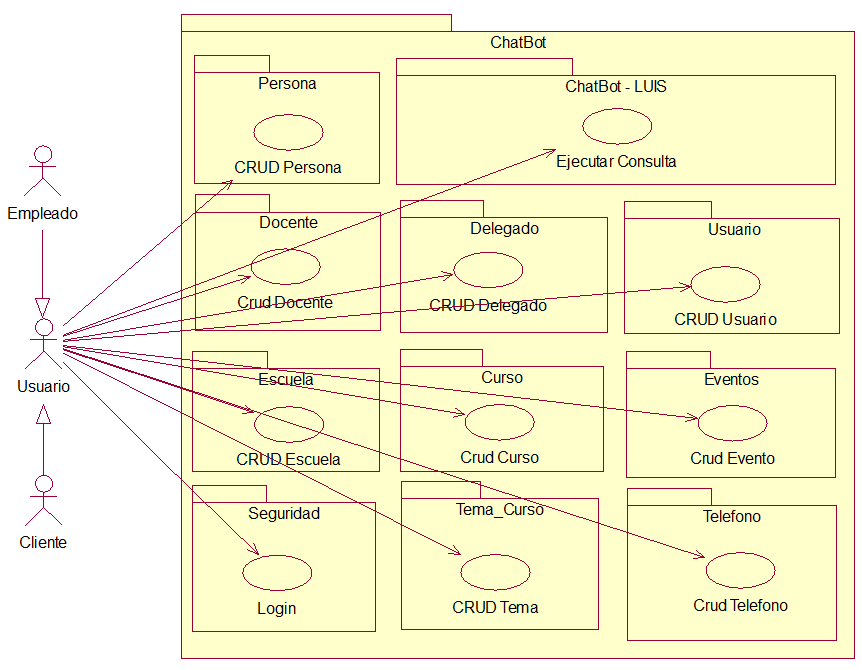
\includegraphics[width=5.07in,height=3.94in]{./media/image7.png}
	\end{Center}
\end{figure}


%%%%%%%%%%%%%%%%%%%% Figure/Image No: 9 Ends here %%%%%%%%%%%%%%%%%%%%

\par



 %%%%%%%%%%%%  Starting New Page here %%%%%%%%%%%%%%

\newpage

\vspace{\baselineskip}\subsection*{7.7\hspace*{10pt}Base Datos:}
\addcontentsline{toc}{subsection}{7.7\hspace*{10pt}Base Datos:}
\begin{itemize}
	\item {\fontsize{10pt}{12.0pt}\selectfont Modelo Entidad/ Relación \par}
\end{itemize}\par



%%%%%%%%%%%%%%%%%%%% Figure/Image No: 10 starts here %%%%%%%%%%%%%%%%%%%%

\begin{figure}[H]
	\begin{FlushLeft}		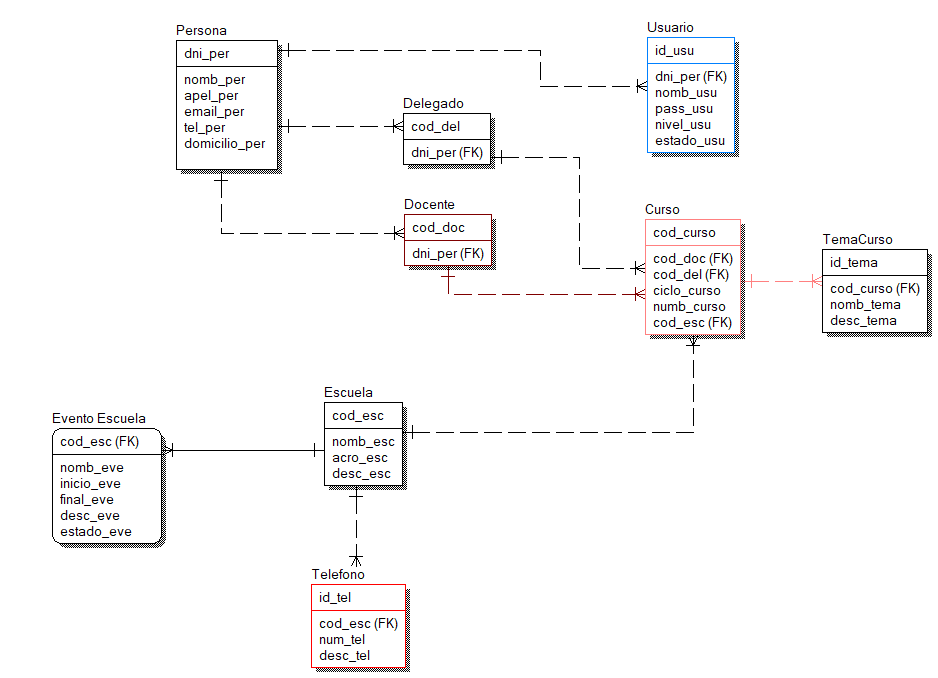
\includegraphics[width=5.94in,height=4.29in]{./media/image8.png}
	\end{FlushLeft}\end{figure}


%%%%%%%%%%%%%%%%%%%% Figure/Image No: 10 Ends here %%%%%%%%%%%%%%%%%%%%

\par

\subsection*{7.8\hspace*{10pt}Diagramas:}
\addcontentsline{toc}{subsection}{7.8\hspace*{10pt}Diagramas:}
\begin{itemize}
	\item {\fontsize{10pt}{12.0pt}\selectfont Diagrama de clases\par}\par

{\fontsize{10pt}{12.0pt}\selectfont \textbf{Persona}\par}\par



%%%%%%%%%%%%%%%%%%%% Figure/Image No: 11 starts here %%%%%%%%%%%%%%%%%%%%

\begin{figure}[H]
	\begin{Center}
		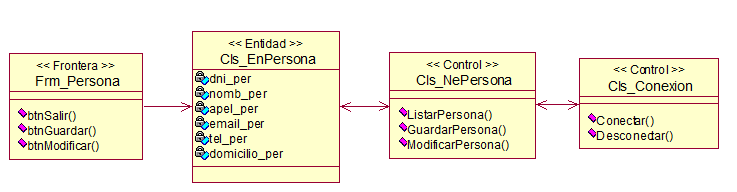
\includegraphics[width=6.33in,height=1.65in]{./media/image9.png}
	\end{Center}
\end{figure}


%%%%%%%%%%%%%%%%%%%% Figure/Image No: 11 Ends here %%%%%%%%%%%%%%%%%%%%

\par



 %%%%%%%%%%%%  Starting New Page here %%%%%%%%%%%%%%

\newpage

\vspace{\baselineskip}{\fontsize{10pt}{12.0pt}\selectfont \textbf{Docente}\par}\par



%%%%%%%%%%%%%%%%%%%% Figure/Image No: 12 starts here %%%%%%%%%%%%%%%%%%%%

\begin{figure}[H]
	\begin{Center}
		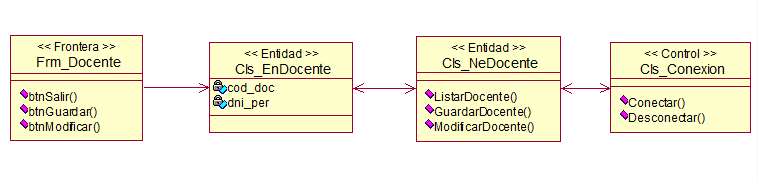
\includegraphics[width=6.33in,height=1.51in]{./media/image10.png}
	\end{Center}
\end{figure}


%%%%%%%%%%%%%%%%%%%% Figure/Image No: 12 Ends here %%%%%%%%%%%%%%%%%%%%

\par

{\fontsize{10pt}{12.0pt}\selectfont \textbf{Delegado}\par}\par



%%%%%%%%%%%%%%%%%%%% Figure/Image No: 13 starts here %%%%%%%%%%%%%%%%%%%%

\begin{figure}[H]
	\begin{Center}
		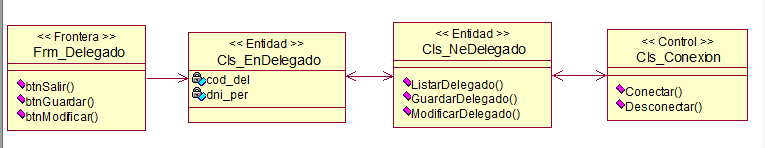
\includegraphics[width=6.29in,height=1.23in]{./media/image11.png}
	\end{Center}
\end{figure}


%%%%%%%%%%%%%%%%%%%% Figure/Image No: 13 Ends here %%%%%%%%%%%%%%%%%%%%

\par

{\fontsize{10pt}{12.0pt}\selectfont \textbf{Usuario}\par}\par



%%%%%%%%%%%%%%%%%%%% Figure/Image No: 14 starts here %%%%%%%%%%%%%%%%%%%%

\begin{figure}[H]
	\begin{Center}
		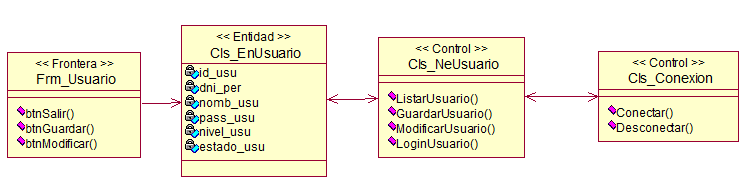
\includegraphics[width=6.33in,height=1.46in]{./media/image12.png}
	\end{Center}
\end{figure}


%%%%%%%%%%%%%%%%%%%% Figure/Image No: 14 Ends here %%%%%%%%%%%%%%%%%%%%

\par

{\fontsize{10pt}{12.0pt}\selectfont \textbf{Escuela}\par}\par



%%%%%%%%%%%%%%%%%%%% Figure/Image No: 15 starts here %%%%%%%%%%%%%%%%%%%%

\begin{figure}[H]
	\begin{Center}
		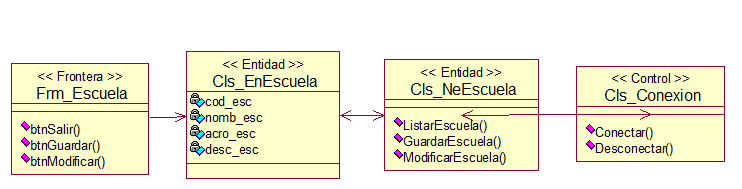
\includegraphics[width=6.33in,height=1.26in]{./media/image13.png}
	\end{Center}
\end{figure}


%%%%%%%%%%%%%%%%%%%% Figure/Image No: 15 Ends here %%%%%%%%%%%%%%%%%%%%

\par

{\fontsize{10pt}{12.0pt}\selectfont \textbf{Curso}\par}\par



%%%%%%%%%%%%%%%%%%%% Figure/Image No: 16 starts here %%%%%%%%%%%%%%%%%%%%

\begin{figure}[H]
	\begin{Center}
		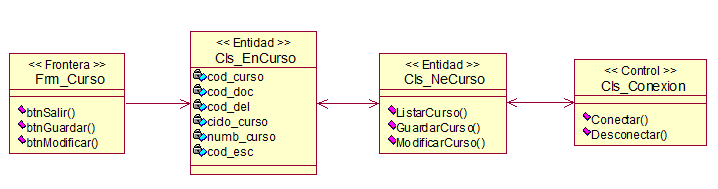
\includegraphics[width=6.33in,height=1.44in]{./media/image14.png}
	\end{Center}
\end{figure}


%%%%%%%%%%%%%%%%%%%% Figure/Image No: 16 Ends here %%%%%%%%%%%%%%%%%%%%

\par


\vspace{\baselineskip}

\vspace{\baselineskip}
{\fontsize{10pt}{12.0pt}\selectfont \textbf{Evento}\par}\par



%%%%%%%%%%%%%%%%%%%% Figure/Image No: 17 starts here %%%%%%%%%%%%%%%%%%%%

\begin{figure}[H]
	\begin{Center}
		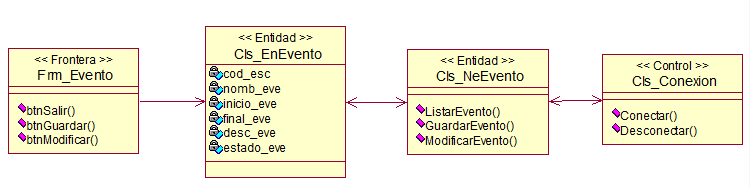
\includegraphics[width=6.33in,height=1.41in]{./media/image15.png}
	\end{Center}
\end{figure}


%%%%%%%%%%%%%%%%%%%% Figure/Image No: 17 Ends here %%%%%%%%%%%%%%%%%%%%

\par

{\fontsize{10pt}{12.0pt}\selectfont \textbf{Tema}\par}\par



%%%%%%%%%%%%%%%%%%%% Figure/Image No: 18 starts here %%%%%%%%%%%%%%%%%%%%

\begin{figure}[H]
	\begin{Center}
		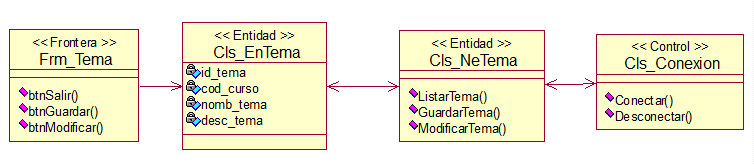
\includegraphics[width=6.33in,height=1.38in]{./media/image16.png}
	\end{Center}
\end{figure}


%%%%%%%%%%%%%%%%%%%% Figure/Image No: 18 Ends here %%%%%%%%%%%%%%%%%%%%

\par

{\fontsize{10pt}{12.0pt}\selectfont \textbf{Teléfono}\par}\par



%%%%%%%%%%%%%%%%%%%% Figure/Image No: 19 starts here %%%%%%%%%%%%%%%%%%%%

\begin{figure}[H]
	\begin{Center}
		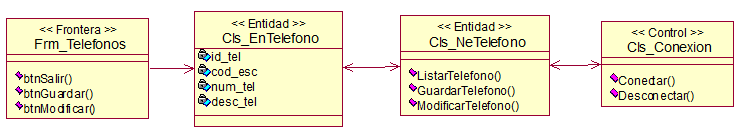
\includegraphics[width=6.33in,height=1.08in]{./media/image17.png}
	\end{Center}
\end{figure}


%%%%%%%%%%%%%%%%%%%% Figure/Image No: 19 Ends here %%%%%%%%%%%%%%%%%%%%

\par

{\fontsize{10pt}{12.0pt}\selectfont \textbf{Login}\par}\par



%%%%%%%%%%%%%%%%%%%% Figure/Image No: 20 starts here %%%%%%%%%%%%%%%%%%%%

\begin{figure}[H]
	\begin{Center}
		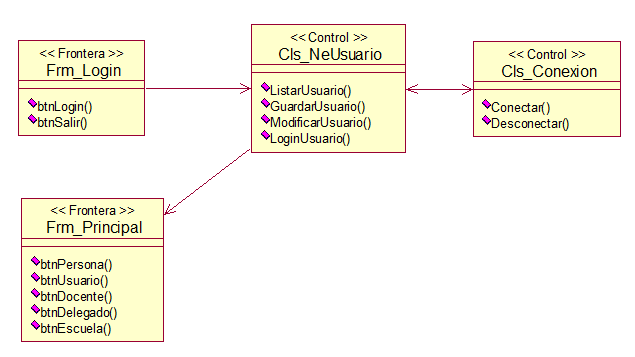
\includegraphics[width=6.33in,height=3.56in]{./media/image18.png}
	\end{Center}
\end{figure}


%%%%%%%%%%%%%%%%%%%% Figure/Image No: 20 Ends here %%%%%%%%%%%%%%%%%%%%

\par


\vspace{\baselineskip}
{\fontsize{10pt}{12.0pt}\selectfont \textbf{ChatBot - LUIS}\par}\par



%%%%%%%%%%%%%%%%%%%% Figure/Image No: 21 starts here %%%%%%%%%%%%%%%%%%%%

\begin{figure}[H]
	\begin{Center}
		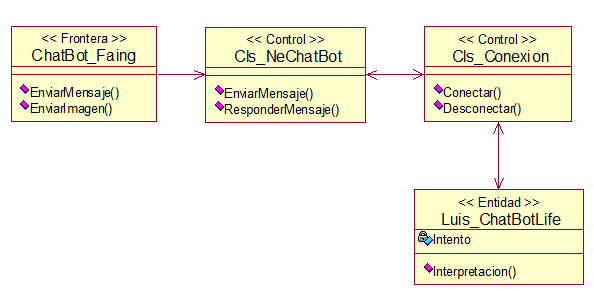
\includegraphics[width=6.19in,height=3.06in]{./media/image19.png}
	\end{Center}
\end{figure}


%%%%%%%%%%%%%%%%%%%% Figure/Image No: 21 Ends here %%%%%%%%%%%%%%%%%%%%

\par


\vspace{\baselineskip}
	\item {\fontsize{10pt}{12.0pt}\selectfont Diagrama de componentes\par}\par



%%%%%%%%%%%%%%%%%%%% Figure/Image No: 22 starts here %%%%%%%%%%%%%%%%%%%%

\begin{figure}[H]
	\begin{Center}
		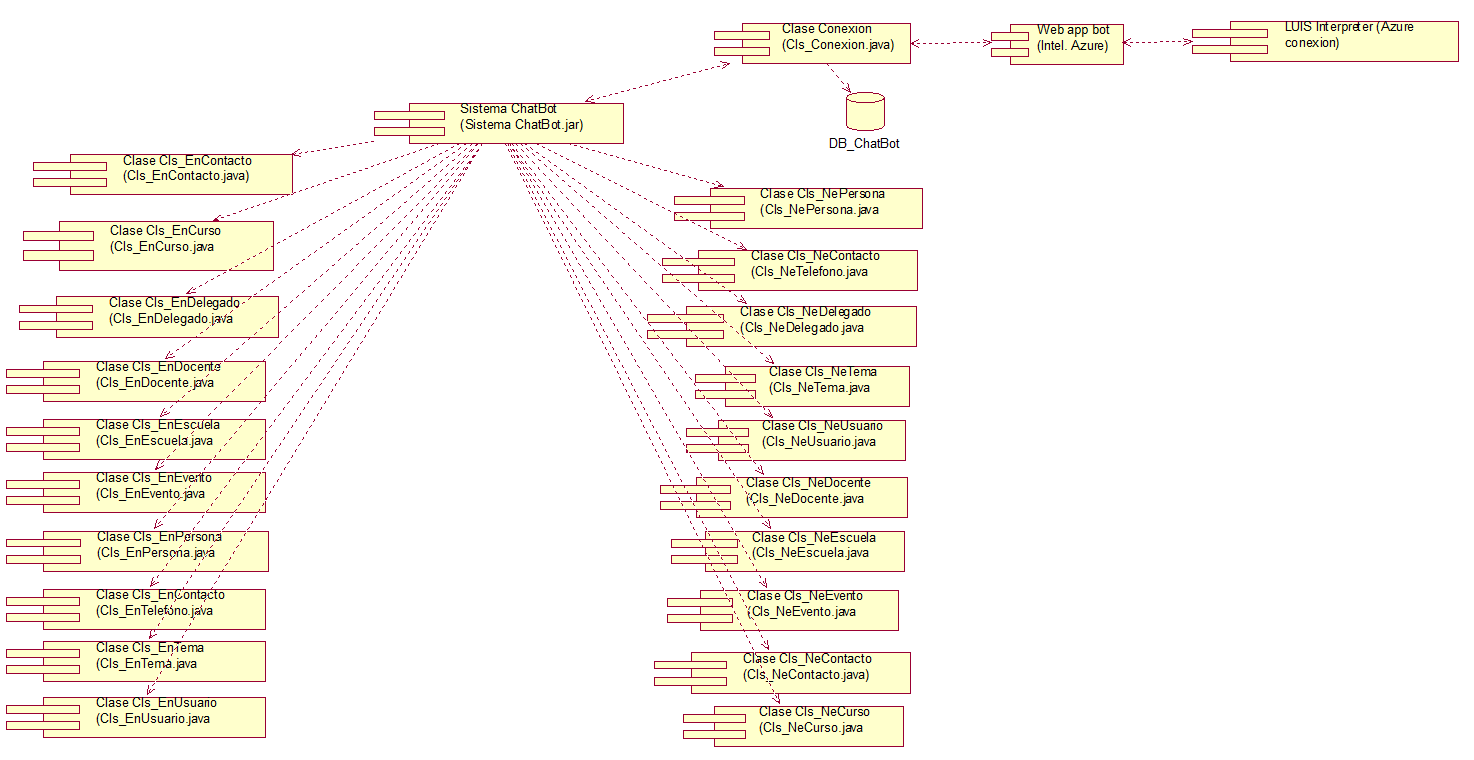
\includegraphics[width=6.33in,height=3.27in]{./media/image20.png}
	\end{Center}
\end{figure}


%%%%%%%%%%%%%%%%%%%% Figure/Image No: 22 Ends here %%%%%%%%%%%%%%%%%%%%

\par


\vspace{\baselineskip}


 %%%%%%%%%%%%  Starting New Page here %%%%%%%%%%%%%%

\newpage

\vspace{\baselineskip}	\item {\fontsize{10pt}{12.0pt}\selectfont Diagrama de Despliegue\par}
\end{itemize}\par



%%%%%%%%%%%%%%%%%%%% Figure/Image No: 23 starts here %%%%%%%%%%%%%%%%%%%%

\begin{figure}[H]
	\begin{Center}
		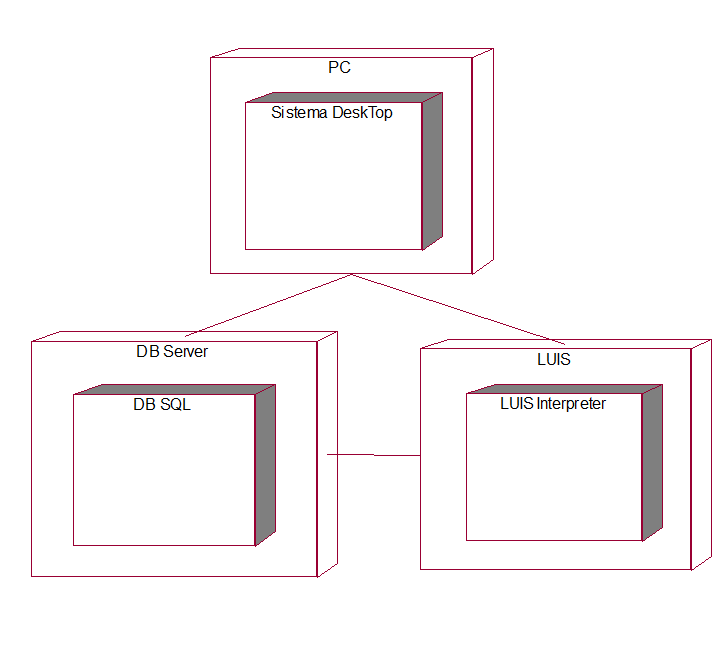
\includegraphics[width=3.98in,height=3.0in]{./media/image21.png}
	\end{Center}
\end{figure}


%%%%%%%%%%%%%%%%%%%% Figure/Image No: 23 Ends here %%%%%%%%%%%%%%%%%%%%

\par

\subsection*{7.9\hspace*{10pt}Arquitectura del Proyecto:}
\addcontentsline{toc}{subsection}{7.9\hspace*{10pt}Arquitectura del Proyecto:}
\begin{itemize}
	\item Descripción de la arquitectura\par

El proyecto se constituye de 2 sistemas.\par

\begin{enumerate}
	\item \textbf{Sistema que gestiona el contenido:}\par

Acá el encargado creara las escuelas, los docentes, otros usuarios, etc. Con la finalidad de poder introducir datos que será mostrados por el chatbot.\par

	\item \textbf{Chatbot:}
\end{enumerate}\par

Se encargra de procesar los mensajes a través de LUIS y según las respuesta se consultara a la base de datos con los datos ingresados en el primer sistema.\par

	\item Desarrollo de los elementos de la arquitectura\par


\vspace{\baselineskip}
\vspace{\baselineskip}

\vspace{\baselineskip}
	\item Diagrama de Arquitectura Técnica
\end{itemize}\par

\par 
 \begin{tikzpicture}

\path (1.58in,-1.97in) node [shape=rectangle,draw,minimum height=3.53in,minimum width=2.2in,]{};
\begin{adjustwidth}{1.0in}{0.0in}
{\fontsize{10pt}{12.0pt}\selectfont Capa cliente\tab \tab \tab \tab \tab \tab Capa presentación\par}\end{adjustwidth}


\path (4.89in,-1.8in) node [shape=rectangle,draw,minimum height=3.53in,minimum width=2.2in,]{};

\end{tikzpicture}


%%%%%%%%%%%%%%%%%%%% Figure/Image No: 24 starts here %%%%%%%%%%%%%%%%%%%%

\begin{figure}[H]
\advance\leftskip 0.9in		
\includegraphics[width=1.47in,height=1.06in]{./media/image22.png}
\end{figure}


%%%%%%%%%%%%%%%%%%%% Figure/Image No: 24 Ends here %%%%%%%%%%%%%%%%%%%%

\par


\vspace{\baselineskip}

\vspace{\baselineskip}

\vspace{\baselineskip}

\vspace{\baselineskip}

\vspace{\baselineskip}
\par 
 \begin{tikzpicture}

\path (4.9in,-0.43in) node [shape=rectangle,draw={rgb:red,0;green,0;blue,0},fill={rgb:red,255;green,255;blue,255},minimum height=0.59in,minimum width=1.65in,text width=1.48in,align=center]{Presentación y desarrollo visual};

\end{tikzpicture}

\vspace{\baselineskip}
\par 
 \begin{tikzpicture}

\end{tikzpicture}

\vspace{\baselineskip}


%%%%%%%%%%%%%%%%%%%% Figure/Image No: 25 starts here %%%%%%%%%%%%%%%%%%%%

\begin{figure}[H]
\advance\leftskip 1.18in		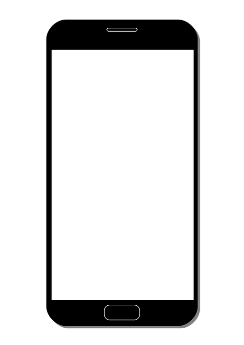
\includegraphics[width=0.72in,height=1.42in]{./media/image23.png}
\end{figure}


%%%%%%%%%%%%%%%%%%%% Figure/Image No: 25 Ends here %%%%%%%%%%%%%%%%%%%%

\par


\vspace{\baselineskip}
\par 
 \begin{tikzpicture}

\end{tikzpicture}

\vspace{\baselineskip}

\vspace{\baselineskip}

\vspace{\baselineskip}

\vspace{\baselineskip}

\vspace{\baselineskip}

\vspace{\baselineskip}

\vspace{\baselineskip}

\vspace{\baselineskip}

\vspace{\baselineskip}
{\fontsize{10pt}{12.0pt}\selectfont Capa de negocio\tab \tab \tab \tab \tab Capa de datos\par}\par

\par 
 \begin{tikzpicture}

\path (4.87in,-1.86in) node [shape=rectangle,draw,minimum height=3.53in,minimum width=2.2in,]{};

\path (1.59in,-1.88in) node [shape=rectangle,draw,minimum height=3.53in,minimum width=2.2in,]{};

\end{tikzpicture}

\vspace{\baselineskip}
\par 
 \begin{tikzpicture}

\path (4.92in,-0.4in) node [shape=rectangle,draw={rgb:red,0;green,0;blue,0},fill={rgb:red,255;green,255;blue,255},minimum height=0.59in,minimum width=1.65in,text width=1.48in,align=center]{Servicio de la nube y Base de datos};

\end{tikzpicture}

\vspace{\baselineskip}
\par 
 \begin{tikzpicture}

\path (1.6in,-0.44in) node [shape=rectangle,draw={rgb:red,0;green,0;blue,0},fill={rgb:red,255;green,255;blue,255},minimum height=0.59in,minimum width=1.65in,text width=1.48in,align=center]{Gestor de mensajes recibidos};

\end{tikzpicture}

\vspace{\baselineskip}

\vspace{\baselineskip}

\vspace{\baselineskip}


%%%%%%%%%%%%%%%%%%%% Figure/Image No: 26 starts here %%%%%%%%%%%%%%%%%%%%

\begin{figure}[H]
\advance\leftskip 4.15in		
\includegraphics[width=1.46in,height=0.82in]{./media/image24.jpeg}
\end{figure}


%%%%%%%%%%%%%%%%%%%% Figure/Image No: 26 Ends here %%%%%%%%%%%%%%%%%%%%

\par

\par 
 \begin{tikzpicture}

\path (1.61in,-0.4in) node [shape=rectangle,draw={rgb:red,0;green,0;blue,0},fill={rgb:red,255;green,255;blue,255},minimum height=0.59in,minimum width=1.65in,text width=1.48in,align=center]{Gestor de respuestas};

\end{tikzpicture}

\vspace{\baselineskip}

\vspace{\baselineskip}

\vspace{\baselineskip}

\vspace{\baselineskip}


%%%%%%%%%%%%%%%%%%%% Figure/Image No: 27 starts here %%%%%%%%%%%%%%%%%%%%


\begin{figure}[H]	\begin{subfigure}		
\includegraphics[width=0.45\textwidth]{./media/image25.png}
	\end{subfigure}
~	\begin{subfigure}		
\includegraphics[width=0.45\textwidth]{./media/image26.png}
	\end{subfigure}
~
\end{figure}


%%%%%%%%%%%%%%%%%%%% Figure/Image No: 27 Ends here %%%%%%%%%%%%%%%%%%%%

\par


\vspace{\baselineskip}

\vspace{\baselineskip}

\vspace{\baselineskip}

\vspace{\baselineskip}

\vspace{\baselineskip}

\vspace{\baselineskip}


 %%%%%%%%%%%%  Starting New Page here %%%%%%%%%%%%%%

\newpage

\vspace{\baselineskip}\setlength{\parskip}{0.0pt}
	\item \textbf{ANEXOS:}\par

\begin{enumerate}
	\item Árbol de Problemas\par

\par 
 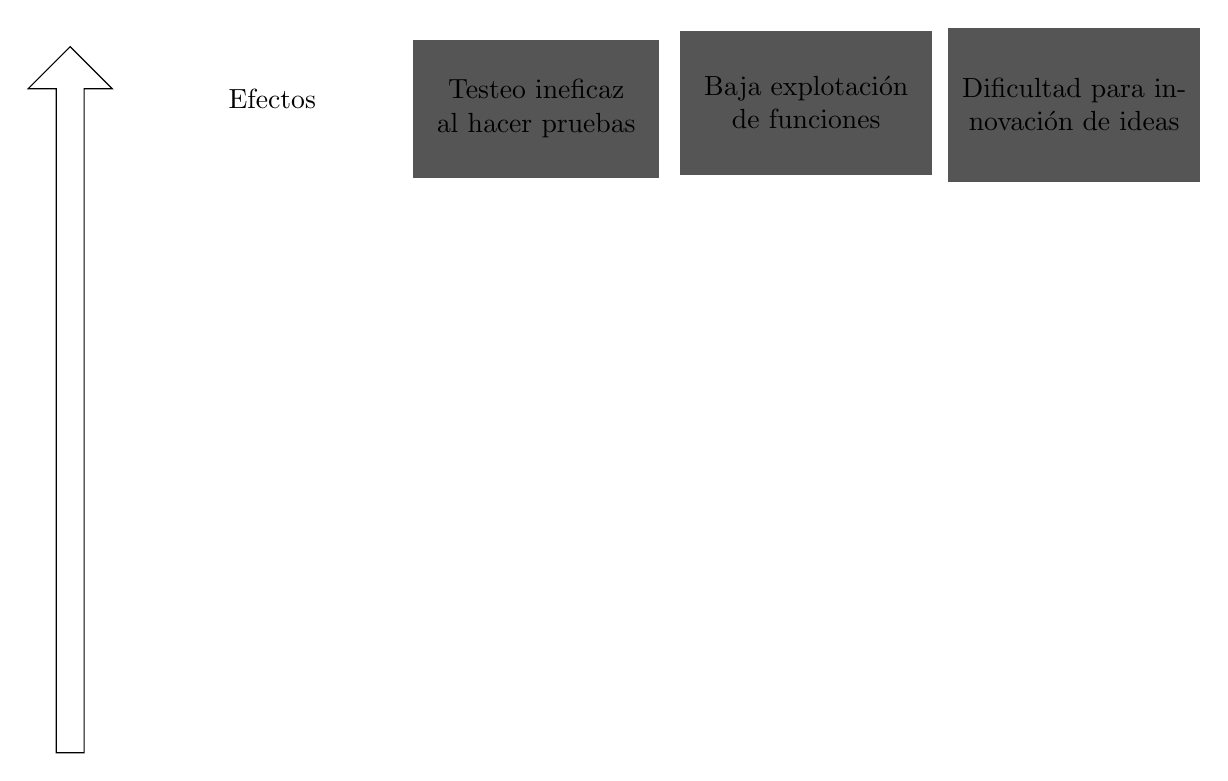
\begin{tikzpicture}

\path (3.26in,-0.45in) node [shape=rectangle,fill={rgb:red,255;green,255;blue,255},minimum height=0.69in,minimum width=1.23in,text width=1.11in,align=center]{Testeo ineficaz al hacer pruebas};

\path (5.95in,-0.43in) node [shape=rectangle,fill={rgb:red,255;green,255;blue,255},minimum height=0.77in,minimum width=1.26in,text width=1.13in,align=center]{Dificultad para innovación de ideas};

\path (4.61in,-0.42in) node [shape=rectangle,fill={rgb:red,255;green,255;blue,255},minimum height=0.72in,minimum width=1.26in,text width=1.13in,align=center]{Baja explotación de funciones};

\path (1.94in,-0.4in) node [shape=rectangle,minimum height=0.54in,minimum width=1.25in,text width=1.12in,align=center]{Efectos};

\path (0.93in,-1.94in) node [shape=single arrow,shape border rotate=90,double arrow head extend=0.14in,draw,minimum height=3.53in,minimum width=0.42in,]{};

\end{tikzpicture}

\vspace{\baselineskip}

\vspace{\baselineskip}
\par 
 
\begin{tikzpicture}

\path (5.92in,-0.32in) node [shape=rectangle,fill={rgb:red,255;green,255;blue,255},minimum height=0.5in,minimum width=1.23in,text width=1.11in,align=center]{Falta de experimentar};

\path (4.58in,-0.31in) node [shape=rectangle,fill={rgb:red,255;green,255;blue,255},minimum height=0.5in,minimum width=1.23in,text width=1.11in,align=center]{Gran cantidad de información};

\path (3.25in,-0.23in) node [shape=rectangle,fill={rgb:red,255;green,255;blue,255},minimum height=0.32in,minimum width=1.23in,text width=1.11in,align=center]{Poca atención};

\end{tikzpicture}

\vspace{\baselineskip}
\par 
 
\begin{tikzpicture}

\path (4.62in,-0.55in) node [shape=rectangle,fill={rgb:red,255;green,255;blue,255},minimum height=0.55in,minimum width=3.85in,text width=3.47in,align=center]{Falta de tiempo para poder investigar nuevas tecnologías para implementar};

\path (1.88in,-0.56in) node [shape=rectangle,fill={rgb:red,192;green,0;blue,0},minimum height=0.58in,minimum width=1.39in,text width=1.25in,align=center]{Problema central};

\end{tikzpicture}

\vspace{\baselineskip}

\vspace{\baselineskip}

\vspace{\baselineskip}

\vspace{\baselineskip}
\par 
 
\begin{tikzpicture}

\path (1.86in,-0.53in) node [shape=rectangle,minimum height=0.5in,minimum width=1.29in,text width=1.16in,align=center]{Causas};

\path (4.52in,-0.27in) node [shape=rectangle,fill={rgb:red,255;green,255;blue,255},minimum height=0.5in,minimum width=0.98in,text width=0.88in,align=center]{Tecnologías nuevas};

\path (5.8in,-0.27in) node [shape=rectangle,fill={rgb:red,255;green,255;blue,255},minimum height=0.5in,minimum width=1.26in,text width=1.13in,align=center]{Carencia de conocimiento};

\path (3.24in,-0.27in) node [shape=rectangle,fill={rgb:red,255;green,255;blue,255},minimum height=0.49in,minimum width=1.26in,text width=1.13in,align=center]{Falta de tiempo};

\end{tikzpicture}

\vspace{\baselineskip}

\vspace{\baselineskip}
	\item Árbol de Objetivos \par

\par 
 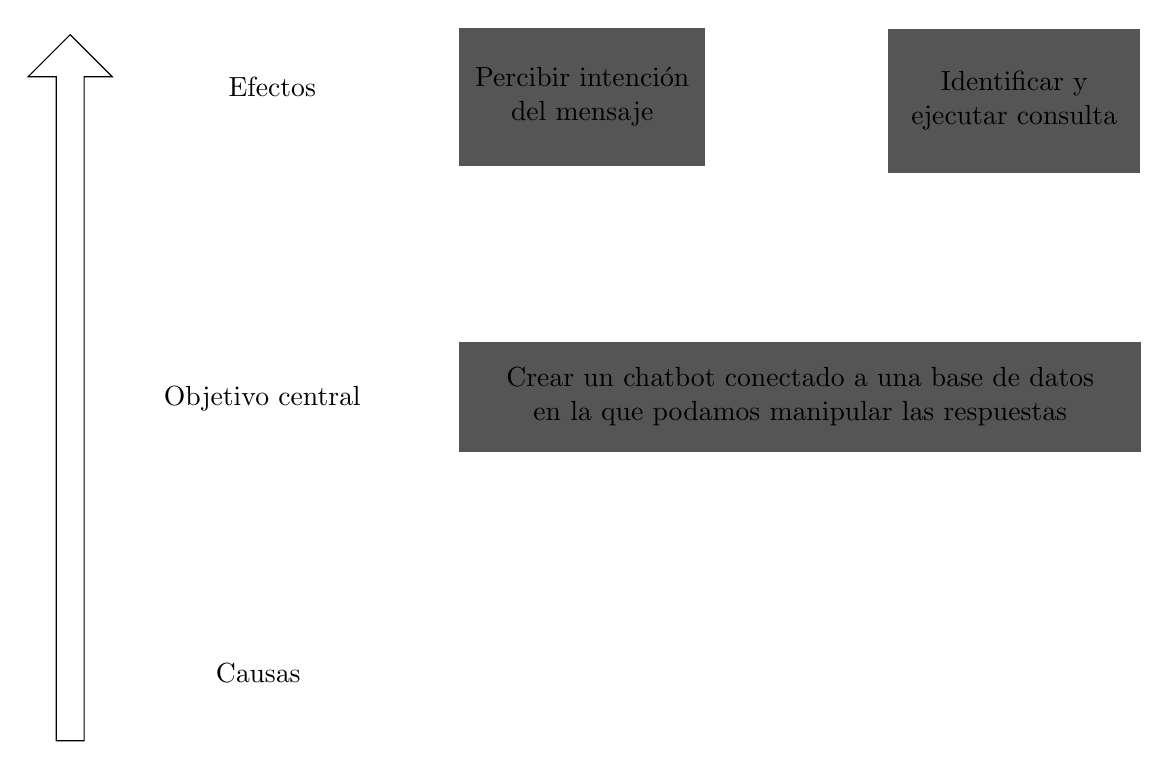
\begin{tikzpicture}

\path (3.54in,-0.44in) node [shape=rectangle,fill={rgb:red,255;green,255;blue,255},minimum height=0.69in,minimum width=1.23in,text width=1.11in,align=center]{Percibir intención del mensaje};

\path (5.7in,-0.46in) node [shape=rectangle,fill={rgb:red,255;green,255;blue,255},minimum height=0.72in,minimum width=1.26in,text width=1.13in,align=center]{Identificar y ejecutar consulta};

\path (4.63in,-1.94in) node [shape=rectangle,fill={rgb:red,255;green,255;blue,255},minimum height=0.55in,minimum width=3.41in,text width=3.07in,align=center]{Crear un chatbot conectado a una base de datos en la que podamos manipular las respuestas};

\path (1.99in,-0.39in) node [shape=rectangle,minimum height=0.54in,minimum width=1.25in,text width=1.12in,align=center]{Efectos};

\path (1.94in,-1.95in) node [shape=rectangle,minimum height=0.58in,minimum width=1.39in,text width=1.25in,align=center]{Objetivo central};

\path (1.92in,-3.32in) node [shape=rectangle,minimum height=0.5in,minimum width=1.29in,text width=1.16in,align=center]{Causas};

\path (0.98in,-1.93in) node [shape=single arrow,shape border rotate=90,double arrow head extend=0.14in,draw,minimum height=3.53in,minimum width=0.42in,]{};

\end{tikzpicture}

\vspace{\baselineskip}

\vspace{\baselineskip}
\par 
 
\begin{tikzpicture}

\path (3.53in,-0.34in) node [shape=rectangle,fill={rgb:red,255;green,255;blue,255},minimum height=0.55in,minimum width=1.23in,text width=1.11in,align=center]{Detectar mensaje};

\path (5.67in,-0.34in) node [shape=rectangle,fill={rgb:red,255;green,255;blue,255},minimum height=0.5in,minimum width=1.23in,text width=1.11in,align=center]{Responder mensaje};

\end{tikzpicture}

\vspace{\baselineskip}

\vspace{\baselineskip}

\vspace{\baselineskip}

\vspace{\baselineskip}

\vspace{\baselineskip}

\vspace{\baselineskip}

\vspace{\baselineskip}
\par 
 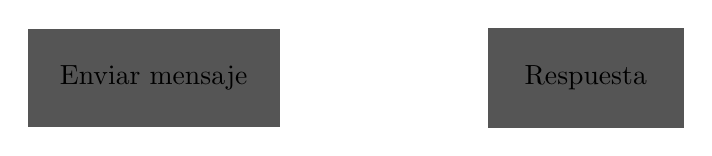
\begin{tikzpicture}

\path (5.68in,-0.26in) node [shape=rectangle,fill={rgb:red,255;green,255;blue,255},minimum height=0.5in,minimum width=0.98in,text width=0.88in,align=center]{Respuesta};

\path (3.52in,-0.26in) node [shape=rectangle,fill={rgb:red,255;green,255;blue,255},minimum height=0.49in,minimum width=1.26in,text width=1.13in,align=center]{Enviar mensaje};

\end{tikzpicture}

\vspace{\baselineskip}

\vspace{\baselineskip}
\setlength{\parskip}{9.96pt}


 %%%%%%%%%%%%  Starting New Page here %%%%%%%%%%%%%%

\newpage

\vspace{\baselineskip}	\item Recursos\par

\begin{itemize}
	\item Convenio Microsoft azure\par

	\item Base de datos Sql Server\par

	\item NetBeans 8.1\par

	\item JDK 1.8
\end{itemize}\par


\vspace{\baselineskip}
	\item Cronograma\par

\textbf{Presentación del avance del equipo}\par



%%%%%%%%%%%%%%%%%%%% Table No: 4 starts here %%%%%%%%%%%%%%%%%%%%


\begin{table}[H]
 			\centering
\begin{tabular}{p{0.51in}p{1.96in}p{2.19in}}
\hline
%row no:1
\multicolumn{1}{|p{0.51in}}{ID} & 
\multicolumn{1}{|p{1.96in}}{Descripción} & 
\multicolumn{1}{|p{2.19in}|}{Fecha/Hora} \\
\hhline{---}
%row no:2
\multicolumn{1}{|p{0.51in}}{1} & 
\multicolumn{1}{|p{1.96in}}{Preparación del proyecto} & 
\multicolumn{1}{|p{2.19in}|}{06/10/2018 10:00} \\
\hhline{---}
%row no:3
\multicolumn{1}{|p{0.51in}}{2} & 
\multicolumn{1}{|p{1.96in}}{Presentación avance 1} & 
\multicolumn{1}{|p{2.19in}|}{11/10/2018 16:00} \\
\hhline{---}
%row no:4
\multicolumn{1}{|p{0.51in}}{3} & 
\multicolumn{1}{|p{1.96in}}{Presentación avance 2} & 
\multicolumn{1}{|p{2.19in}|}{18/10/2018 15:00} \\
\hhline{---}
%row no:5
\multicolumn{1}{|p{0.51in}}{4} & 
\multicolumn{1}{|p{1.96in}}{Presentación avance 3} & 
\multicolumn{1}{|p{2.19in}|}{25/10/2018 16:00} \\
\hhline{---}
%row no:6
\multicolumn{1}{|p{0.51in}}{5} & 
\multicolumn{1}{|p{1.96in}}{Entrega del Proyecto final} & 
\multicolumn{1}{|p{2.19in}|}{30/10/2018 15:00} \\
\hhline{---}

\end{tabular}
 \end{table}


%%%%%%%%%%%%%%%%%%%% Table No: 4 ends here %%%%%%%%%%%%%%%%%%%%


\vspace{\baselineskip}
\textbf{Reunión del equipo}\par



%%%%%%%%%%%%%%%%%%%% Table No: 5 starts here %%%%%%%%%%%%%%%%%%%%


\begin{table}[H]
 			\centering
\begin{tabular}{p{0.51in}p{1.96in}p{2.19in}}
\hline
%row no:1
\multicolumn{1}{|p{0.51in}}{ID} & 
\multicolumn{1}{|p{1.96in}}{Descripción} & 
\multicolumn{1}{|p{2.19in}|}{Fecha/Hora} \\
\hhline{---}
%row no:2
\multicolumn{1}{|p{0.51in}}{1} & 
\multicolumn{1}{|p{1.96in}}{Preparación del proyecto} & 
\multicolumn{1}{|p{2.19in}|}{06/10/2018 10:00} \\
\hhline{---}
%row no:3
\multicolumn{1}{|p{0.51in}}{2} & 
\multicolumn{1}{|p{1.96in}}{Decisión del proyecto} & 
\multicolumn{1}{|p{2.19in}|}{13/10/2018 11:00} \\
\hhline{---}
%row no:4
\multicolumn{1}{|p{0.51in}}{3} & 
\multicolumn{1}{|p{1.96in}}{Creación de la DB y el Sistema desktop} & 
\multicolumn{1}{|p{2.19in}|}{18/10/2018 10:00} \\
\hhline{---}
%row no:5
\multicolumn{1}{|p{0.51in}}{4} & 
\multicolumn{1}{|p{1.96in}}{Implementación del chato} & 
\multicolumn{1}{|p{2.19in}|}{20/10/2018 10:00} \\
\hhline{---}
%row no:6
\multicolumn{1}{|p{0.51in}}{5} & 
\multicolumn{1}{|p{1.96in}}{Documentación y testeo} & 
\multicolumn{1}{|p{2.19in}|}{27/10/2018 10:00} \\
\hhline{---}

\end{tabular}
 \end{table}


%%%%%%%%%%%%%%%%%%%% Table No: 5 ends here %%%%%%%%%%%%%%%%%%%%


\vspace{\baselineskip}


 %%%%%%%%%%%%  Starting New Page here %%%%%%%%%%%%%%

\newpage

\vspace{\baselineskip}	\item Manual de Usuario\par


\vspace{\baselineskip}
	\item Diccionario de Datos\par



%%%%%%%%%%%%%%%%%%%% Table No: 6 starts here %%%%%%%%%%%%%%%%%%%%


\begin{table}[H]
 			\centering
\begin{tabular}{p{0.3in}p{0.67in}p{0.5in}p{0.48in}p{0.7in}p{2.17in}}
\hline
%row no:1
\multicolumn{6}{|p{5.82in}|}{	\item {\fontsize{10pt}{12.0pt}\selectfont PERSONA}} \\
\hhline{------}
%row no:2
\multicolumn{1}{|p{0.3in}}{{\fontsize{10pt}{12.0pt}\selectfont LLAVE}} & 
\multicolumn{1}{|p{0.67in}}{{\fontsize{10pt}{12.0pt}\selectfont ATRIBUTO}} & 
\multicolumn{1}{|p{0.5in}}{{\fontsize{10pt}{12.0pt}\selectfont TIPO}} & 
\multicolumn{1}{|p{0.48in}}{{\fontsize{10pt}{12.0pt}\selectfont TAMAÑO}} & 
\multicolumn{1}{|p{0.7in}}{{\fontsize{10pt}{12.0pt}\selectfont RESTRICCION}} & 
\multicolumn{1}{|p{2.17in}|}{{\fontsize{10pt}{12.0pt}\selectfont DESCRIPCION}} \\
\hhline{------}
%row no:3
\multicolumn{1}{|p{0.3in}}{{\fontsize{10pt}{12.0pt}\selectfont PK}} & 
\multicolumn{1}{|p{0.67in}}{{\fontsize{10pt}{12.0pt}\selectfont DniPersona}} & 
\multicolumn{1}{|p{0.5in}}{{\fontsize{10pt}{12.0pt}\selectfont VarChar}} & 
\multicolumn{1}{|p{0.48in}}{{\fontsize{10pt}{12.0pt}\selectfont 10}} & 
\multicolumn{1}{|p{0.7in}}{{\fontsize{10pt}{12.0pt}\selectfont Not Null}} & 
\multicolumn{1}{|p{2.17in}|}{{\fontsize{10pt}{12.0pt}\selectfont Almacena el DNI de la Persona}} \\
\hhline{------}
%row no:4
\multicolumn{1}{|p{0.3in}}{} & 
\multicolumn{1}{|p{0.67in}}{{\fontsize{10pt}{12.0pt}\selectfont NombPer}} & 
\multicolumn{1}{|p{0.5in}}{{\fontsize{10pt}{12.0pt}\selectfont VarChar}} & 
\multicolumn{1}{|p{0.48in}}{{\fontsize{10pt}{12.0pt}\selectfont 250}} & 
\multicolumn{1}{|p{0.7in}}{{\fontsize{10pt}{12.0pt}\selectfont Not Null}} & 
\multicolumn{1}{|p{2.17in}|}{{\fontsize{10pt}{12.0pt}\selectfont Almacena el Nombre de la Persona}} \\
\hhline{------}
%row no:5
\multicolumn{1}{|p{0.3in}}{} & 
\multicolumn{1}{|p{0.67in}}{{\fontsize{10pt}{12.0pt}\selectfont ApelPer}} & 
\multicolumn{1}{|p{0.5in}}{{\fontsize{10pt}{12.0pt}\selectfont VarChar}} & 
\multicolumn{1}{|p{0.48in}}{{\fontsize{10pt}{12.0pt}\selectfont 250}} & 
\multicolumn{1}{|p{0.7in}}{{\fontsize{10pt}{12.0pt}\selectfont Not Null}} & 
\multicolumn{1}{|p{2.17in}|}{{\fontsize{10pt}{12.0pt}\selectfont Almacena el Apellido de la Persona}} \\
\hhline{------}
%row no:6
\multicolumn{1}{|p{0.3in}}{} & 
\multicolumn{1}{|p{0.67in}}{{\fontsize{10pt}{12.0pt}\selectfont EmailPer}} & 
\multicolumn{1}{|p{0.5in}}{{\fontsize{10pt}{12.0pt}\selectfont VarChar}} & 
\multicolumn{1}{|p{0.48in}}{{\fontsize{10pt}{12.0pt}\selectfont 250}} & 
\multicolumn{1}{|p{0.7in}}{{\fontsize{10pt}{12.0pt}\selectfont Not Null}} & 
\multicolumn{1}{|p{2.17in}|}{{\fontsize{10pt}{12.0pt}\selectfont Almacena la Email de la Persona}} \\
\hhline{------}
%row no:7
\multicolumn{1}{|p{0.3in}}{} & 
\multicolumn{1}{|p{0.67in}}{{\fontsize{10pt}{12.0pt}\selectfont TelPer}} & 
\multicolumn{1}{|p{0.5in}}{{\fontsize{10pt}{12.0pt}\selectfont VarChar}} & 
\multicolumn{1}{|p{0.48in}}{{\fontsize{10pt}{12.0pt}\selectfont 11}} & 
\multicolumn{1}{|p{0.7in}}{{\fontsize{10pt}{12.0pt}\selectfont Not Null}} & 
\multicolumn{1}{|p{2.17in}|}{{\fontsize{10pt}{12.0pt}\selectfont Almacena el Telefono de la Persona}} \\
\hhline{------}
%row no:8
\multicolumn{1}{|p{0.3in}}{} & 
\multicolumn{1}{|p{0.67in}}{{\fontsize{10pt}{12.0pt}\selectfont DomicilioPer}} & 
\multicolumn{1}{|p{0.5in}}{{\fontsize{10pt}{12.0pt}\selectfont VarChar}} & 
\multicolumn{1}{|p{0.48in}}{{\fontsize{10pt}{12.0pt}\selectfont 250}} & 
\multicolumn{1}{|p{0.7in}}{{\fontsize{10pt}{12.0pt}\selectfont Not Null}} & 
\multicolumn{1}{|p{2.17in}|}{{\fontsize{10pt}{12.0pt}\selectfont Almacena el Domicilio de la Persona}} \\
\hhline{------}

\end{tabular}
 \end{table}


%%%%%%%%%%%%%%%%%%%% Table No: 6 ends here %%%%%%%%%%%%%%%%%%%%


\vspace{\baselineskip}


%%%%%%%%%%%%%%%%%%%% Table No: 7 starts here %%%%%%%%%%%%%%%%%%%%


\begin{table}[H]
 			\centering
\begin{tabular}{p{0.3in}p{0.56in}p{0.5in}p{0.48in}p{0.7in}p{2.27in}}
\hline
%row no:1
\multicolumn{6}{|p{5.81in}|}{\Centering USUARIO} \\
\hhline{------}
%row no:2
\multicolumn{1}{|p{0.3in}}{{\fontsize{10pt}{12.0pt}\selectfont LLAVE}} & 
\multicolumn{1}{|p{0.56in}}{{\fontsize{10pt}{12.0pt}\selectfont ATRIBUTO}} & 
\multicolumn{1}{|p{0.5in}}{{\fontsize{10pt}{12.0pt}\selectfont TIPO}} & 
\multicolumn{1}{|p{0.48in}}{{\fontsize{10pt}{12.0pt}\selectfont TAMAÑO}} & 
\multicolumn{1}{|p{0.7in}}{{\fontsize{10pt}{12.0pt}\selectfont RESTRICCION}} & 
\multicolumn{1}{|p{2.27in}|}{{\fontsize{10pt}{12.0pt}\selectfont DESCRIPCION}} \\
\hhline{------}
%row no:3
\multicolumn{1}{|p{0.3in}}{{\fontsize{10pt}{12.0pt}\selectfont PK}} & 
\multicolumn{1}{|p{0.56in}}{{\fontsize{10pt}{12.0pt}\selectfont IdUsu}} & 
\multicolumn{1}{|p{0.5in}}{{\fontsize{10pt}{12.0pt}\selectfont Int}} & 
\multicolumn{1}{|p{0.48in}}{{\fontsize{10pt}{12.0pt}\selectfont 11}} & 
\multicolumn{1}{|p{0.7in}}{{\fontsize{10pt}{12.0pt}\selectfont Null}} & 
\multicolumn{1}{|p{2.27in}|}{{\fontsize{10pt}{12.0pt}\selectfont Almacena el Id del Usuario}} \\
\hhline{------}
%row no:4
\multicolumn{1}{|p{0.3in}}{{\fontsize{10pt}{12.0pt}\selectfont FK}} & 
\multicolumn{1}{|p{0.56in}}{{\fontsize{10pt}{12.0pt}\selectfont DniPer}} & 
\multicolumn{1}{|p{0.5in}}{{\fontsize{10pt}{12.0pt}\selectfont VarChar}} & 
\multicolumn{1}{|p{0.48in}}{{\fontsize{10pt}{12.0pt}\selectfont 10}} & 
\multicolumn{1}{|p{0.7in}}{{\fontsize{10pt}{12.0pt}\selectfont Not Null}} & 
\multicolumn{1}{|p{2.27in}|}{{\fontsize{10pt}{12.0pt}\selectfont Almacena el Dni de la Persona}} \\
\hhline{------}
%row no:5
\multicolumn{1}{|p{0.3in}}{} & 
\multicolumn{1}{|p{0.56in}}{{\fontsize{10pt}{12.0pt}\selectfont NombUsu}} & 
\multicolumn{1}{|p{0.5in}}{{\fontsize{10pt}{12.0pt}\selectfont VarChar}} & 
\multicolumn{1}{|p{0.48in}}{{\fontsize{10pt}{12.0pt}\selectfont 50}} & 
\multicolumn{1}{|p{0.7in}}{{\fontsize{10pt}{12.0pt}\selectfont Not Null}} & 
\multicolumn{1}{|p{2.27in}|}{{\fontsize{10pt}{12.0pt}\selectfont Almacena el nombre de usuario}} \\
\hhline{------}
%row no:6
\multicolumn{1}{|p{0.3in}}{} & 
\multicolumn{1}{|p{0.56in}}{{\fontsize{10pt}{12.0pt}\selectfont PassUsu}} & 
\multicolumn{1}{|p{0.5in}}{{\fontsize{10pt}{12.0pt}\selectfont VarChar}} & 
\multicolumn{1}{|p{0.48in}}{{\fontsize{10pt}{12.0pt}\selectfont 80}} & 
\multicolumn{1}{|p{0.7in}}{{\fontsize{10pt}{12.0pt}\selectfont Null}} & 
\multicolumn{1}{|p{2.27in}|}{{\fontsize{10pt}{12.0pt}\selectfont Almacena la contraseña del usuario}} \\
\hhline{------}
%row no:7
\multicolumn{1}{|p{0.3in}}{} & 
\multicolumn{1}{|p{0.56in}}{{\fontsize{10pt}{12.0pt}\selectfont NivelUsu}} & 
\multicolumn{1}{|p{0.5in}}{{\fontsize{10pt}{12.0pt}\selectfont VarChar}} & 
\multicolumn{1}{|p{0.48in}}{{\fontsize{10pt}{12.0pt}\selectfont 10}} & 
\multicolumn{1}{|p{0.7in}}{{\fontsize{10pt}{12.0pt}\selectfont Null}} & 
\multicolumn{1}{|p{2.27in}|}{{\fontsize{10pt}{12.0pt}\selectfont Almacena el Nivel del Usuario}} \\
\hhline{------}
%row no:8
\multicolumn{1}{|p{0.3in}}{} & 
\multicolumn{1}{|p{0.56in}}{{\fontsize{10pt}{12.0pt}\selectfont EstadoUsu}} & 
\multicolumn{1}{|p{0.5in}}{{\fontsize{10pt}{12.0pt}\selectfont VarChar}} & 
\multicolumn{1}{|p{0.48in}}{{\fontsize{10pt}{12.0pt}\selectfont 10}} & 
\multicolumn{1}{|p{0.7in}}{{\fontsize{10pt}{12.0pt}\selectfont Null}} & 
\multicolumn{1}{|p{2.27in}|}{{\fontsize{10pt}{12.0pt}\selectfont Almacena el Estado del Usuario}} \\
\hhline{------}

\end{tabular}
 \end{table}


%%%%%%%%%%%%%%%%%%%% Table No: 7 ends here %%%%%%%%%%%%%%%%%%%%


\vspace{\baselineskip}


%%%%%%%%%%%%%%%%%%%% Table No: 8 starts here %%%%%%%%%%%%%%%%%%%%


\begin{table}[H]
 			\centering
\begin{tabular}{p{0.3in}p{0.9in}p{0.54in}p{0.49in}p{0.7in}p{1.92in}}
\hline
%row no:1
\multicolumn{6}{|p{5.86in}|}{\Centering DOCENTE} \\
\hhline{------}
%row no:2
\multicolumn{1}{|p{0.3in}}{{\fontsize{10pt}{12.0pt}\selectfont LLAVE}} & 
\multicolumn{1}{|p{0.9in}}{{\fontsize{10pt}{12.0pt}\selectfont ATRIBUTO}} & 
\multicolumn{1}{|p{0.54in}}{{\fontsize{10pt}{12.0pt}\selectfont TIPO}} & 
\multicolumn{1}{|p{0.49in}}{{\fontsize{10pt}{12.0pt}\selectfont TAMAÑO}} & 
\multicolumn{1}{|p{0.7in}}{{\fontsize{10pt}{12.0pt}\selectfont RESTRICCION}} & 
\multicolumn{1}{|p{1.92in}|}{{\fontsize{10pt}{12.0pt}\selectfont DESCRIPCION}} \\
\hhline{------}
%row no:3
\multicolumn{1}{|p{0.3in}}{{\fontsize{10pt}{12.0pt}\selectfont PK}} & 
\multicolumn{1}{|p{0.9in}}{{\fontsize{10pt}{12.0pt}\selectfont CodDoc}} & 
\multicolumn{1}{|p{0.54in}}{{\fontsize{10pt}{12.0pt}\selectfont VarChar}} & 
\multicolumn{1}{|p{0.49in}}{{\fontsize{10pt}{12.0pt}\selectfont 10}} & 
\multicolumn{1}{|p{0.7in}}{{\fontsize{10pt}{12.0pt}\selectfont Not Null}} & 
\multicolumn{1}{|p{1.92in}|}{{\fontsize{10pt}{12.0pt}\selectfont Almacena el Codigo del Docente}} \\
\hhline{------}
%row no:4
\multicolumn{1}{|p{0.3in}}{{\fontsize{10pt}{12.0pt}\selectfont FK}} & 
\multicolumn{1}{|p{0.9in}}{{\fontsize{10pt}{12.0pt}\selectfont DniPer}} & 
\multicolumn{1}{|p{0.54in}}{{\fontsize{10pt}{12.0pt}\selectfont VarChar}} & 
\multicolumn{1}{|p{0.49in}}{{\fontsize{10pt}{12.0pt}\selectfont 10}} & 
\multicolumn{1}{|p{0.7in}}{{\fontsize{10pt}{12.0pt}\selectfont Not Null}} & 
\multicolumn{1}{|p{1.92in}|}{{\fontsize{10pt}{12.0pt}\selectfont Almacena el Dni de la Persona}} \\
\hhline{------}

\end{tabular}
 \end{table}


%%%%%%%%%%%%%%%%%%%% Table No: 8 ends here %%%%%%%%%%%%%%%%%%%%


\vspace{\baselineskip}


%%%%%%%%%%%%%%%%%%%% Table No: 9 starts here %%%%%%%%%%%%%%%%%%%%


\begin{table}[H]
 			\centering
\begin{tabular}{p{0.3in}p{0.9in}p{0.54in}p{0.49in}p{0.7in}p{1.92in}}
\hline
%row no:1
\multicolumn{6}{|p{5.86in}|}{\Centering DELEGADO} \\
\hhline{------}
%row no:2
\multicolumn{1}{|p{0.3in}}{{\fontsize{10pt}{12.0pt}\selectfont LLAVE}} & 
\multicolumn{1}{|p{0.9in}}{{\fontsize{10pt}{12.0pt}\selectfont ATRIBUTO}} & 
\multicolumn{1}{|p{0.54in}}{{\fontsize{10pt}{12.0pt}\selectfont TIPO}} & 
\multicolumn{1}{|p{0.49in}}{{\fontsize{10pt}{12.0pt}\selectfont TAMAÑO}} & 
\multicolumn{1}{|p{0.7in}}{{\fontsize{10pt}{12.0pt}\selectfont RESTRICCION}} & 
\multicolumn{1}{|p{1.92in}|}{{\fontsize{10pt}{12.0pt}\selectfont DESCRIPCION}} \\
\hhline{------}
%row no:3
\multicolumn{1}{|p{0.3in}}{{\fontsize{10pt}{12.0pt}\selectfont PK}} & 
\multicolumn{1}{|p{0.9in}}{{\fontsize{10pt}{12.0pt}\selectfont CodDel}} & 
\multicolumn{1}{|p{0.54in}}{{\fontsize{10pt}{12.0pt}\selectfont VarChar}} & 
\multicolumn{1}{|p{0.49in}}{{\fontsize{10pt}{12.0pt}\selectfont 10}} & 
\multicolumn{1}{|p{0.7in}}{{\fontsize{10pt}{12.0pt}\selectfont Not Null}} & 
\multicolumn{1}{|p{1.92in}|}{{\fontsize{10pt}{12.0pt}\selectfont Almacena el Codigo del Delegado}} \\
\hhline{------}
%row no:4
\multicolumn{1}{|p{0.3in}}{{\fontsize{10pt}{12.0pt}\selectfont FK}} & 
\multicolumn{1}{|p{0.9in}}{{\fontsize{10pt}{12.0pt}\selectfont DniPer}} & 
\multicolumn{1}{|p{0.54in}}{{\fontsize{10pt}{12.0pt}\selectfont VarChar}} & 
\multicolumn{1}{|p{0.49in}}{{\fontsize{10pt}{12.0pt}\selectfont 10}} & 
\multicolumn{1}{|p{0.7in}}{{\fontsize{10pt}{12.0pt}\selectfont Not Null}} & 
\multicolumn{1}{|p{1.92in}|}{{\fontsize{10pt}{12.0pt}\selectfont Almacena el Dni de la Persona}} \\
\hhline{------}

\end{tabular}
 \end{table}


%%%%%%%%%%%%%%%%%%%% Table No: 9 ends here %%%%%%%%%%%%%%%%%%%%


\vspace{\baselineskip}

\vspace{\baselineskip}

\vspace{\baselineskip}


%%%%%%%%%%%%%%%%%%%% Table No: 10 starts here %%%%%%%%%%%%%%%%%%%%


\begin{table}[H]
 			\centering
\begin{tabular}{p{0.3in}p{0.68in}p{0.5in}p{0.48in}p{0.7in}p{2.15in}}
\hline
%row no:1
\multicolumn{6}{|p{5.81in}|}{\Centering ESCUELA} \\
\hhline{------}
%row no:2
\multicolumn{1}{|p{0.3in}}{{\fontsize{10pt}{12.0pt}\selectfont LLAVE}} & 
\multicolumn{1}{|p{0.68in}}{{\fontsize{10pt}{12.0pt}\selectfont ATRIBUTO}} & 
\multicolumn{1}{|p{0.5in}}{{\fontsize{10pt}{12.0pt}\selectfont TIPO}} & 
\multicolumn{1}{|p{0.48in}}{{\fontsize{10pt}{12.0pt}\selectfont TAMAÑO}} & 
\multicolumn{1}{|p{0.7in}}{{\fontsize{10pt}{12.0pt}\selectfont RESTRICCION}} & 
\multicolumn{1}{|p{2.15in}|}{{\fontsize{10pt}{12.0pt}\selectfont DESCRIPCION}} \\
\hhline{------}
%row no:3
\multicolumn{1}{|p{0.3in}}{{\fontsize{10pt}{12.0pt}\selectfont PK}} & 
\multicolumn{1}{|p{0.68in}}{{\fontsize{10pt}{12.0pt}\selectfont CodEsc}} & 
\multicolumn{1}{|p{0.5in}}{{\fontsize{10pt}{12.0pt}\selectfont VarChar}} & 
\multicolumn{1}{|p{0.48in}}{{\fontsize{10pt}{12.0pt}\selectfont 10}} & 
\multicolumn{1}{|p{0.7in}}{{\fontsize{10pt}{12.0pt}\selectfont Not Null}} & 
\multicolumn{1}{|p{2.15in}|}{{\fontsize{10pt}{12.0pt}\selectfont Almacena el Codigo de la Escuela}} \\
\hhline{------}
%row no:4
\multicolumn{1}{|p{0.3in}}{} & 
\multicolumn{1}{|p{0.68in}}{{\fontsize{10pt}{12.0pt}\selectfont NombEsc}} & 
\multicolumn{1}{|p{0.5in}}{{\fontsize{10pt}{12.0pt}\selectfont VarChar}} & 
\multicolumn{1}{|p{0.48in}}{{\fontsize{10pt}{12.0pt}\selectfont 250}} & 
\multicolumn{1}{|p{0.7in}}{{\fontsize{10pt}{12.0pt}\selectfont Not Null}} & 
\multicolumn{1}{|p{2.15in}|}{{\fontsize{10pt}{12.0pt}\selectfont Almacena el Nombre de la Escuela}} \\
\hhline{------}
%row no:5
\multicolumn{1}{|p{0.3in}}{} & 
\multicolumn{1}{|p{0.68in}}{{\fontsize{10pt}{12.0pt}\selectfont AcroEsc}} & 
\multicolumn{1}{|p{0.5in}}{{\fontsize{10pt}{12.0pt}\selectfont VarChar}} & 
\multicolumn{1}{|p{0.48in}}{{\fontsize{10pt}{12.0pt}\selectfont 10}} & 
\multicolumn{1}{|p{0.7in}}{{\fontsize{10pt}{12.0pt}\selectfont Not Null}} & 
\multicolumn{1}{|p{2.15in}|}{{\fontsize{10pt}{12.0pt}\selectfont Almacena el Acronimo de la Escuela}} \\
\hhline{------}
%row no:6
\multicolumn{1}{|p{0.3in}}{} & 
\multicolumn{1}{|p{0.68in}}{{\fontsize{10pt}{12.0pt}\selectfont DescEsc}} & 
\multicolumn{1}{|p{0.5in}}{{\fontsize{10pt}{12.0pt}\selectfont VarChar}} & 
\multicolumn{1}{|p{0.48in}}{{\fontsize{10pt}{12.0pt}\selectfont 250}} & 
\multicolumn{1}{|p{0.7in}}{{\fontsize{10pt}{12.0pt}\selectfont Not Null}} & 
\multicolumn{1}{|p{2.15in}|}{{\fontsize{10pt}{12.0pt}\selectfont Almacena la Descripcion de la Escuela}} \\
\hhline{------}

\end{tabular}
 \end{table}


%%%%%%%%%%%%%%%%%%%% Table No: 10 ends here %%%%%%%%%%%%%%%%%%%%


\vspace{\baselineskip}


%%%%%%%%%%%%%%%%%%%% Table No: 11 starts here %%%%%%%%%%%%%%%%%%%%


\begin{table}[H]
 			\centering
\begin{tabular}{p{0.3in}p{0.56in}p{0.5in}p{0.48in}p{0.7in}p{2.27in}}
\hline
%row no:1
\multicolumn{6}{|p{5.81in}|}{\Centering EVENTO} \\
\hhline{------}
%row no:2
\multicolumn{1}{|p{0.3in}}{{\fontsize{10pt}{12.0pt}\selectfont LLAVE}} & 
\multicolumn{1}{|p{0.56in}}{{\fontsize{10pt}{12.0pt}\selectfont ATRIBUTO}} & 
\multicolumn{1}{|p{0.5in}}{{\fontsize{10pt}{12.0pt}\selectfont TIPO}} & 
\multicolumn{1}{|p{0.48in}}{{\fontsize{10pt}{12.0pt}\selectfont TAMAÑO}} & 
\multicolumn{1}{|p{0.7in}}{{\fontsize{10pt}{12.0pt}\selectfont RESTRICCION}} & 
\multicolumn{1}{|p{2.27in}|}{{\fontsize{10pt}{12.0pt}\selectfont DESCRIPCION}} \\
\hhline{------}
%row no:3
\multicolumn{1}{|p{0.3in}}{{\fontsize{10pt}{12.0pt}\selectfont PK}} & 
\multicolumn{1}{|p{0.56in}}{{\fontsize{10pt}{12.0pt}\selectfont CodEsc}} & 
\multicolumn{1}{|p{0.5in}}{{\fontsize{10pt}{12.0pt}\selectfont VarChar}} & 
\multicolumn{1}{|p{0.48in}}{{\fontsize{10pt}{12.0pt}\selectfont 10}} & 
\multicolumn{1}{|p{0.7in}}{{\fontsize{10pt}{12.0pt}\selectfont Not Null}} & 
\multicolumn{1}{|p{2.27in}|}{{\fontsize{10pt}{12.0pt}\selectfont Almacena el Codigo de la Escuela}} \\
\hhline{------}
%row no:4
\multicolumn{1}{|p{0.3in}}{} & 
\multicolumn{1}{|p{0.56in}}{{\fontsize{10pt}{12.0pt}\selectfont NombEve}} & 
\multicolumn{1}{|p{0.5in}}{{\fontsize{10pt}{12.0pt}\selectfont VarChar}} & 
\multicolumn{1}{|p{0.48in}}{{\fontsize{10pt}{12.0pt}\selectfont 50}} & 
\multicolumn{1}{|p{0.7in}}{{\fontsize{10pt}{12.0pt}\selectfont Not Null}} & 
\multicolumn{1}{|p{2.27in}|}{{\fontsize{10pt}{12.0pt}\selectfont Almacena el Nombre del Evento}} \\
\hhline{------}
%row no:5
\multicolumn{1}{|p{0.3in}}{} & 
\multicolumn{1}{|p{0.56in}}{{\fontsize{10pt}{12.0pt}\selectfont InicioEve}} & 
\multicolumn{1}{|p{0.5in}}{{\fontsize{10pt}{12.0pt}\selectfont Date}} & 
\multicolumn{1}{|p{0.48in}}{{\fontsize{10pt}{12.0pt}\selectfont $\ast$ }} & 
\multicolumn{1}{|p{0.7in}}{{\fontsize{10pt}{12.0pt}\selectfont Not Null}} & 
\multicolumn{1}{|p{2.27in}|}{{\fontsize{10pt}{12.0pt}\selectfont Almacena el Inicio del Evento}} \\
\hhline{------}
%row no:6
\multicolumn{1}{|p{0.3in}}{} & 
\multicolumn{1}{|p{0.56in}}{{\fontsize{10pt}{12.0pt}\selectfont FinalEve}} & 
\multicolumn{1}{|p{0.5in}}{{\fontsize{10pt}{12.0pt}\selectfont Date}} & 
\multicolumn{1}{|p{0.48in}}{{\fontsize{10pt}{12.0pt}\selectfont $\ast$ }} & 
\multicolumn{1}{|p{0.7in}}{{\fontsize{10pt}{12.0pt}\selectfont Not Null}} & 
\multicolumn{1}{|p{2.27in}|}{{\fontsize{10pt}{12.0pt}\selectfont Almacena el Final del Evento}} \\
\hhline{------}
%row no:7
\multicolumn{1}{|p{0.3in}}{} & 
\multicolumn{1}{|p{0.56in}}{{\fontsize{10pt}{12.0pt}\selectfont DescEve}} & 
\multicolumn{1}{|p{0.5in}}{{\fontsize{10pt}{12.0pt}\selectfont VarChar}} & 
\multicolumn{1}{|p{0.48in}}{{\fontsize{10pt}{12.0pt}\selectfont 250}} & 
\multicolumn{1}{|p{0.7in}}{{\fontsize{10pt}{12.0pt}\selectfont Not Null}} & 
\multicolumn{1}{|p{2.27in}|}{{\fontsize{10pt}{12.0pt}\selectfont Almacena la Descripcion del Evento}} \\
\hhline{------}
%row no:8
\multicolumn{1}{|p{0.3in}}{} & 
\multicolumn{1}{|p{0.56in}}{{\fontsize{10pt}{12.0pt}\selectfont EstadoEve}} & 
\multicolumn{1}{|p{0.5in}}{{\fontsize{10pt}{12.0pt}\selectfont VarChar}} & 
\multicolumn{1}{|p{0.48in}}{{\fontsize{10pt}{12.0pt}\selectfont 10}} & 
\multicolumn{1}{|p{0.7in}}{{\fontsize{10pt}{12.0pt}\selectfont Null}} & 
\multicolumn{1}{|p{2.27in}|}{{\fontsize{10pt}{12.0pt}\selectfont Almacena el Estado del Evento}} \\
\hhline{------}

\end{tabular}
 \end{table}


%%%%%%%%%%%%%%%%%%%% Table No: 11 ends here %%%%%%%%%%%%%%%%%%%%


\vspace{\baselineskip}


%%%%%%%%%%%%%%%%%%%% Table No: 12 starts here %%%%%%%%%%%%%%%%%%%%


\begin{table}[H]
 			\centering
\begin{tabular}{p{0.3in}p{0.76in}p{0.41in}p{0.48in}p{0.7in}p{2.16in}}
\hline
%row no:1
\multicolumn{6}{|p{5.81in}|}{\Centering TELEFONO} \\
\hhline{------}
%row no:2
\multicolumn{1}{|p{0.3in}}{{\fontsize{10pt}{12.0pt}\selectfont LLAVE}} & 
\multicolumn{1}{|p{0.76in}}{{\fontsize{10pt}{12.0pt}\selectfont ATRIBUTO}} & 
\multicolumn{1}{|p{0.41in}}{{\fontsize{10pt}{12.0pt}\selectfont TIPO}} & 
\multicolumn{1}{|p{0.48in}}{{\fontsize{10pt}{12.0pt}\selectfont TAMAÑO}} & 
\multicolumn{1}{|p{0.7in}}{{\fontsize{10pt}{12.0pt}\selectfont RESTRICCION}} & 
\multicolumn{1}{|p{2.16in}|}{{\fontsize{10pt}{12.0pt}\selectfont DESCRIPCION}} \\
\hhline{------}
%row no:3
\multicolumn{1}{|p{0.3in}}{{\fontsize{10pt}{12.0pt}\selectfont PK}} & 
\multicolumn{1}{|p{0.76in}}{{\fontsize{10pt}{12.0pt}\selectfont IdTel}} & 
\multicolumn{1}{|p{0.41in}}{{\fontsize{10pt}{12.0pt}\selectfont Int}} & 
\multicolumn{1}{|p{0.48in}}{{\fontsize{10pt}{12.0pt}\selectfont $\ast$ }} & 
\multicolumn{1}{|p{0.7in}}{{\fontsize{10pt}{12.0pt}\selectfont Not Null}} & 
\multicolumn{1}{|p{2.16in}|}{{\fontsize{10pt}{12.0pt}\selectfont Identificador de Laboratorio}} \\
\hhline{------}
%row no:4
\multicolumn{1}{|p{0.3in}}{} & 
\multicolumn{1}{|p{0.76in}}{{\fontsize{10pt}{12.0pt}\selectfont NumTel}} & 
\multicolumn{1}{|p{0.41in}}{{\fontsize{10pt}{12.0pt}\selectfont VarChar}} & 
\multicolumn{1}{|p{0.48in}}{{\fontsize{10pt}{12.0pt}\selectfont 11}} & 
\multicolumn{1}{|p{0.7in}}{{\fontsize{10pt}{12.0pt}\selectfont Not Null}} & 
\multicolumn{1}{|p{2.16in}|}{{\fontsize{10pt}{12.0pt}\selectfont Numero de Telefono}} \\
\hhline{------}
%row no:5
\multicolumn{1}{|p{0.3in}}{{\fontsize{10pt}{12.0pt}\selectfont FK}} & 
\multicolumn{1}{|p{0.76in}}{{\fontsize{10pt}{12.0pt}\selectfont CodEsc}} & 
\multicolumn{1}{|p{0.41in}}{{\fontsize{10pt}{12.0pt}\selectfont VarChar}} & 
\multicolumn{1}{|p{0.48in}}{{\fontsize{10pt}{12.0pt}\selectfont 10}} & 
\multicolumn{1}{|p{0.7in}}{{\fontsize{10pt}{12.0pt}\selectfont Not Null}} & 
\multicolumn{1}{|p{2.16in}|}{{\fontsize{10pt}{12.0pt}\selectfont Codigo de la Escuela}} \\
\hhline{------}
%row no:6
\multicolumn{1}{|p{0.3in}}{} & 
\multicolumn{1}{|p{0.76in}}{{\fontsize{10pt}{12.0pt}\selectfont DescTel}} & 
\multicolumn{1}{|p{0.41in}}{{\fontsize{10pt}{12.0pt}\selectfont VarChar}} & 
\multicolumn{1}{|p{0.48in}}{{\fontsize{10pt}{12.0pt}\selectfont 250}} & 
\multicolumn{1}{|p{0.7in}}{{\fontsize{10pt}{12.0pt}\selectfont Null}} & 
\multicolumn{1}{|p{2.16in}|}{{\fontsize{10pt}{12.0pt}\selectfont Descripcion del Telefono}} \\
\hhline{------}

\end{tabular}
 \end{table}


%%%%%%%%%%%%%%%%%%%% Table No: 12 ends here %%%%%%%%%%%%%%%%%%%%


\vspace{\baselineskip}


%%%%%%%%%%%%%%%%%%%% Table No: 13 starts here %%%%%%%%%%%%%%%%%%%%


\begin{table}[H]
 			\centering
\begin{tabular}{p{0.3in}p{1.0in}p{0.5in}p{0.48in}p{0.75in}p{1.84in}}
\hline
%row no:1
\multicolumn{6}{|p{5.86in}|}{\Centering CURSO} \\
\hhline{------}
%row no:2
\multicolumn{1}{|p{0.3in}}{{\fontsize{10pt}{12.0pt}\selectfont LLAVE}} & 
\multicolumn{1}{|p{1.0in}}{{\fontsize{10pt}{12.0pt}\selectfont ATRIBUTO}} & 
\multicolumn{1}{|p{0.5in}}{{\fontsize{10pt}{12.0pt}\selectfont TIPO}} & 
\multicolumn{1}{|p{0.48in}}{{\fontsize{10pt}{12.0pt}\selectfont TAMAÑO}} & 
\multicolumn{1}{|p{0.75in}}{{\fontsize{10pt}{12.0pt}\selectfont RESTRICCION}} & 
\multicolumn{1}{|p{1.84in}|}{{\fontsize{10pt}{12.0pt}\selectfont DESCRIPCION}} \\
\hhline{------}
%row no:3
\multicolumn{1}{|p{0.3in}}{{\fontsize{10pt}{12.0pt}\selectfont PK}} & 
\multicolumn{1}{|p{1.0in}}{{\fontsize{10pt}{12.0pt}\selectfont CodCurso}} & 
\multicolumn{1}{|p{0.5in}}{{\fontsize{10pt}{12.0pt}\selectfont VarChar}} & 
\multicolumn{1}{|p{0.48in}}{{\fontsize{10pt}{12.0pt}\selectfont 10}} & 
\multicolumn{1}{|p{0.75in}}{{\fontsize{10pt}{12.0pt}\selectfont Not Null}} & 
\multicolumn{1}{|p{1.84in}|}{{\fontsize{10pt}{12.0pt}\selectfont Almacena el Codigo del Curso}} \\
\hhline{------}
%row no:4
\multicolumn{1}{|p{0.3in}}{} & 
\multicolumn{1}{|p{1.0in}}{{\fontsize{10pt}{12.0pt}\selectfont CicloCurso}} & 
\multicolumn{1}{|p{0.5in}}{{\fontsize{10pt}{12.0pt}\selectfont VarChar}} & 
\multicolumn{1}{|p{0.48in}}{{\fontsize{10pt}{12.0pt}\selectfont 10}} & 
\multicolumn{1}{|p{0.75in}}{{\fontsize{10pt}{12.0pt}\selectfont Not Null}} & 
\multicolumn{1}{|p{1.84in}|}{{\fontsize{10pt}{12.0pt}\selectfont Almacena el Ciclo del Curso}} \\
\hhline{------}
%row no:5
\multicolumn{1}{|p{0.3in}}{} & 
\multicolumn{1}{|p{1.0in}}{{\fontsize{10pt}{12.0pt}\selectfont NombCurso}} & 
\multicolumn{1}{|p{0.5in}}{{\fontsize{10pt}{12.0pt}\selectfont VarChar}} & 
\multicolumn{1}{|p{0.48in}}{{\fontsize{10pt}{12.0pt}\selectfont 50}} & 
\multicolumn{1}{|p{0.75in}}{{\fontsize{10pt}{12.0pt}\selectfont Not Null}} & 
\multicolumn{1}{|p{1.84in}|}{{\fontsize{10pt}{12.0pt}\selectfont Almacena el Nombre del Curso}} \\
\hhline{------}
%row no:6
\multicolumn{1}{|p{0.3in}}{{\fontsize{10pt}{12.0pt}\selectfont FK}} & 
\multicolumn{1}{|p{1.0in}}{{\fontsize{10pt}{12.0pt}\selectfont CodDoc}} & 
\multicolumn{1}{|p{0.5in}}{{\fontsize{10pt}{12.0pt}\selectfont VarChar}} & 
\multicolumn{1}{|p{0.48in}}{{\fontsize{10pt}{12.0pt}\selectfont 10}} & 
\multicolumn{1}{|p{0.75in}}{{\fontsize{10pt}{12.0pt}\selectfont Not Null}} & 
\multicolumn{1}{|p{1.84in}|}{{\fontsize{10pt}{12.0pt}\selectfont Almacena el Codigo del Docente}} \\
\hhline{------}
%row no:7
\multicolumn{1}{|p{0.3in}}{{\fontsize{10pt}{12.0pt}\selectfont FK}} & 
\multicolumn{1}{|p{1.0in}}{{\fontsize{10pt}{12.0pt}\selectfont CodDel}} & 
\multicolumn{1}{|p{0.5in}}{{\fontsize{10pt}{12.0pt}\selectfont VarChar}} & 
\multicolumn{1}{|p{0.48in}}{{\fontsize{10pt}{12.0pt}\selectfont 10}} & 
\multicolumn{1}{|p{0.75in}}{{\fontsize{10pt}{12.0pt}\selectfont Null}} & 
\multicolumn{1}{|p{1.84in}|}{{\fontsize{10pt}{12.0pt}\selectfont Almacena el Codigo del Delegado}} \\
\hhline{------}
%row no:8
\multicolumn{1}{|p{0.3in}}{{\fontsize{10pt}{12.0pt}\selectfont FK}} & 
\multicolumn{1}{|p{1.0in}}{{\fontsize{10pt}{12.0pt}\selectfont CodEsc}} & 
\multicolumn{1}{|p{0.5in}}{{\fontsize{10pt}{12.0pt}\selectfont VarChar}} & 
\multicolumn{1}{|p{0.48in}}{{\fontsize{10pt}{12.0pt}\selectfont 10}} & 
\multicolumn{1}{|p{0.75in}}{{\fontsize{10pt}{12.0pt}\selectfont Not Null}} & 
\multicolumn{1}{|p{1.84in}|}{{\fontsize{10pt}{12.0pt}\selectfont Almacena el Codigo de la Escuela}} \\
\hhline{------}

\end{tabular}
 \end{table}


%%%%%%%%%%%%%%%%%%%% Table No: 13 ends here %%%%%%%%%%%%%%%%%%%%


\vspace{\baselineskip}

\vspace{\baselineskip}


%%%%%%%%%%%%%%%%%%%% Table No: 14 starts here %%%%%%%%%%%%%%%%%%%%


\begin{table}[H]
 			\centering
\begin{tabular}{p{0.3in}p{0.75in}p{0.59in}p{-0.05in}p{0.48in}p{0.75in}p{1.84in}}
\hline
%row no:1
\multicolumn{7}{|p{5.86in}|}{\Centering TEMA} \\
\hhline{-------}
%row no:2
\multicolumn{1}{|p{0.3in}}{{\fontsize{10pt}{12.0pt}\selectfont LLAVE}} & 
\multicolumn{1}{|p{0.75in}}{{\fontsize{10pt}{12.0pt}\selectfont ATRIBUTO}} & 
\multicolumn{1}{|p{0.59in}}{{\fontsize{10pt}{12.0pt}\selectfont TIPO}} & 
\multicolumn{2}{|p{0.63in}}{{\fontsize{10pt}{12.0pt}\selectfont TAMAÑO}} & 
\multicolumn{1}{|p{0.75in}}{{\fontsize{10pt}{12.0pt}\selectfont RESTRICCION}} & 
\multicolumn{1}{|p{1.84in}|}{{\fontsize{10pt}{12.0pt}\selectfont DESCRIPCION}} \\
\hhline{-------}
%row no:3
\multicolumn{1}{|p{0.3in}}{{\fontsize{10pt}{12.0pt}\selectfont PK}} & 
\multicolumn{1}{|p{0.75in}}{{\fontsize{10pt}{12.0pt}\selectfont IdTema}} & 
\multicolumn{2}{|p{0.74in}}{{\fontsize{10pt}{12.0pt}\selectfont Int}} & 
\multicolumn{1}{|p{0.48in}}{{\fontsize{10pt}{12.0pt}\selectfont $\ast$ }} & 
\multicolumn{1}{|p{0.75in}}{{\fontsize{10pt}{12.0pt}\selectfont Not Null}} & 
\multicolumn{1}{|p{1.84in}|}{{\fontsize{10pt}{12.0pt}\selectfont Almacena la ID del Tema}} \\
\hhline{-------}
%row no:4
\multicolumn{1}{|p{0.3in}}{{\fontsize{10pt}{12.0pt}\selectfont FK}} & 
\multicolumn{1}{|p{0.75in}}{{\fontsize{10pt}{12.0pt}\selectfont CodCurso}} & 
\multicolumn{2}{|p{0.74in}}{{\fontsize{10pt}{12.0pt}\selectfont VarChar}} & 
\multicolumn{1}{|p{0.48in}}{{\fontsize{10pt}{12.0pt}\selectfont 10}} & 
\multicolumn{1}{|p{0.75in}}{{\fontsize{10pt}{12.0pt}\selectfont Not Null}} & 
\multicolumn{1}{|p{1.84in}|}{{\fontsize{10pt}{12.0pt}\selectfont Almacena el Codigo del Curso}} \\
\hhline{-------}
%row no:5
\multicolumn{1}{|p{0.3in}}{} & 
\multicolumn{1}{|p{0.75in}}{{\fontsize{10pt}{12.0pt}\selectfont NombTema}} & 
\multicolumn{2}{|p{0.74in}}{{\fontsize{10pt}{12.0pt}\selectfont VarChar}} & 
\multicolumn{1}{|p{0.48in}}{{\fontsize{10pt}{12.0pt}\selectfont 50}} & 
\multicolumn{1}{|p{0.75in}}{{\fontsize{10pt}{12.0pt}\selectfont Not Null}} & 
\multicolumn{1}{|p{1.84in}|}{{\fontsize{10pt}{12.0pt}\selectfont Almacena el Nombre del Tema}} \\
\hhline{-------}
%row no:6
\multicolumn{1}{|p{0.3in}}{} & 
\multicolumn{1}{|p{0.75in}}{{\fontsize{10pt}{12.0pt}\selectfont DescTema}} & 
\multicolumn{2}{|p{0.74in}}{{\fontsize{10pt}{12.0pt}\selectfont VarChar}} & 
\multicolumn{1}{|p{0.48in}}{{\fontsize{10pt}{12.0pt}\selectfont 250}} & 
\multicolumn{1}{|p{0.75in}}{{\fontsize{10pt}{12.0pt}\selectfont Not Null}} & 
\multicolumn{1}{|p{1.84in}|}{{\fontsize{10pt}{12.0pt}\selectfont Almacena la Descripcion del Tema}} \\
\hhline{-------}

\end{tabular}
 \end{table}


%%%%%%%%%%%%%%%%%%%% Table No: 14 ends here %%%%%%%%%%%%%%%%%%%%


\vspace{\baselineskip}

\vspace{\baselineskip}
	\item Artículo Científico
\end{enumerate}\par

{\fontsize{10pt}{12.0pt}\selectfont \textbf{\uline{Archivo adjunto}}\par}\par


\printbibliography
\end{document}
